\chapter{Orthogonal Electric Field Measurements near the Green Fluorescent Protein Fluorophore through Stark Effect Spectroscopy and \pKa{} Shifts Provide a Unique Benchmark for Electrostatics Models} \label{gfp-pKa}

Measurement of the magnitude, direction, and functional importance of electric fields in biomolecules has been a longstanding experimental challenge. 
\pKa{} shifts of titratable residues have been the most widely implemented measurements of local electrostatic environment around the labile proton, and experimental data sets of \pKa{} shifts in a variety of systems have been used to test and refine computational prediction capabilities of protein electrostatic fields. 
A more direct and increasingly popular technique to measure electric fields in proteins is Stark effect spectroscopy, where the change in absorption energy of a chromophore relative to a reference state is related to the change in electric field felt by the chromophore. While there are merits to both of these methods and they are both reporters of local electrostatic environment, they are fundamentally different measurements, and to our knowledge there has been no direct comparison of these two approaches in a single protein. 
We have recently demonstrated that green fluorescent protein (GFP) is an ideal model system for measuring changes in electric fields in a protein interior caused by amino acid mutations using both electronic and vibrational Stark effect chromophores. 
Here we report the changes in \pKa{} of the GFP fluorophore in response to the same mutations and show that they are in excellent agreement with Stark effect measurements. 
This agreement in the results of orthogonal experiments reinforces our confidence in the experimental results of both Stark effect and \pKa{} measurements, and provides an excellent target dataset to benchmark diverse protein electrostatics calculations. 
We used this experimental dataset to test the \pKa{} prediction ability of the Adaptive Poisson-Boltzmann Solver (APBS) and found that a simple continuum dielectric model of the GFP interior is insufficient to accurately capture the measured \pKa{} and Stark effect shifts . 
We discuss some of the limitations of this continuum-based model in this system and offer this experimentally self-consistent dataset as a target benchmark for electrostatics models, which could allow for a more rigorous test of \pKa{} prediction techniques due to the unique environment of the water-filled GFP barrel compared to traditional globular proteins.


%%%%%%%%%%%%%%%%%%%%%%%%%%%%%%%%%%%%%%%%%%%%%%%%%%%%%%%%%%%%%%%%
%%%%%%%%%%%%%%%%%%%%%%%%%%%%%%%%%%%%%%%%%%%%%%%%%%%%%%%%%%%%%%%%
\section{Introduction} \label{introduction}
%%%%%%%%%%%%%%%%%%%%%%%%%%%%%%%%%%%%%%%%%%%%%%%%%%%%%%%%%%%%%%%%
%%%%%%%%%%%%%%%%%%%%%%%%%%%%%%%%%%%%%%%%%%%%%%%%%%%%%%%%%%%%%%%%

Electrostatic fields have long been recognized as a key driving force behind all protein functions, including folding, stability, noncovalent interactions with small molecules or large biological macromolecules, catalysis, and other reactivity \cite{Hayes1976, Warshel1978, Honig1995, Gunner1996, Warshel1998}.
Because electric fields generated by the arrangement of partial charges in the structure of a protein are long-range, the electrostatic environment of a protein can be quite complex at the molecular length scale. 
This makes characterizing the magnitude and effect of electric fields in biological molecules a difficult task from both experimental and computational perspectives. 
The most widely implemented experimental technique used to measure electrostatic effects in proteins has been quantifying the perturbation of \pKa{} values of titratable amino acid side chains compared to their values in aqueous buffer \cite{Forsyth2002, Langsetmo1991, Isom2010, Bradbury1966, Markley1975}.
The three-dimensional arrangement and connectivity of partially charged atoms near the titratable residue creates an electrostatic environment that strongly influences the relative stability of charged versus neutral side chains. 
Because of this, the measurement of the equilibrium between these two states is often thought to be a good reporter of the local electrostatic environment around the amino acid. 
\pKa{} values can be measured straightforwardly by recording the pH-dependence of a signal that changes with protonation state; this is commonly done by measuring chemical shifts of labile $^1$H or nearby $^{13}$C atoms by NMR \cite{Markley1975}. 
Experiments like these have led to the estimation of dielectric constants of globular proteins \cite{Dwyer2000, Chimenti2011}, helped rationalize the catalytic mechanisms of enzymes \cite{Inoue1992, Davoodi1995, McIntosh1996}, and have led to an understanding of how charged amino acids can be accommodated in the interior of proteins \cite{Isom2010, Chimenti2011, Isom2008}.

While these \pKa{} values are excellent reporters of the overall electrostatic environment around the titratable residue, it is typically very difficult to rationalize which specific interactions contribute most significantly to the observed equilibrium. 
For instance, lysine, whose side chain \pKa{} is $\sim$10.5 in water, often titrates with a significantly lower \pKa{} when buried in the non-polar interior of a protein. 
This is due to the overall energetic favorability of the non-polar protein environment to contain the neutral form of lysine rather than the charged form. 
However, without further experimental and theoretical investigations, the perturbed \pKa{} values of lysine residues do not offer significant information with molecular level detail of the specific electrostatic interactions that cause the \pKa{} shift.  

Because of the sensitivity of \pKa{} values of titratable amino acid side chains to the overall electrostatic environment around the amino acid, one significant aspect of accurate \pKa{} measurements in proteins is their usefulness as benchmarks for electrostatics models \cite{Gibas1996, Antosiewicz1996, Fogolari2002, Li2005, Olsson2011, Witham2011, Meyer2015, Mehler1999}.
However, this sensitivity can also be viewed as a drawback for modeling, because of the necessity to accurately model long range interactions in a complex protein environment. 
Many attempts have been made to predict the \pKa{} values of different amino acids in proteins to validate electrostatics models with levels of theory ranging from fully atomistic quantum mechanics, to mixed quantum mechanics, to continuum electrostatics \cite{Gibas1996, Antosiewicz1996, Schutz2001, Warshel2006, Nielsen2011}.
However, because of the complexity of electrostatic environments in proteins, the accurate modeling of electrostatic effects often requires excessive computational cost or a vast oversimplification of the relevant physics. 
Most electrostatics models can adequately reproduce the \pKa{} values of solvent exposed side chains that experience negligible shifts in \pKa{} relative to their values in water, but the successful calculation of perturbed \pKa{} values of buried residues, which have been observed to shift by as much as 5 \pKa{} units, is much more difficult \cite{Schutz2001, Simonson2001}.
This requires an accurate and detailed treatment of the complex environment of a protein interior, including dynamic fluctuationsequilibrium sampling \cite{Schutz2001, Nielsen2011, Warshel2011, Alexov2011, Li2013}.

Many current strategies for calculating \pKa{} shifts in proteins involve the use of a thermodynamic cycle to calculate the change in free energy when the titratable residue in question is transferred from water to the protein environment \cite{Fogolari2002, Gorham2011, Getahun2003}.
The strategy taken to accurately calculate these electrostatic free energies is where many common models deviate, although most are based on continuum electrostatics models such as the Poisson-Boltzmann (PB) equation. 
Algorithms to generate distributions of charge states and starting structures for the energy calculations generally increase the agreement with experiment, which suggests that protein fluctuations and charge state coupling is important \cite{Witham2011, Meyer2015}.
However, regardless of the approach, electrostatics models still do a poor job at reproducing \pKa{} shifts of buried residues. 
Indeed, in a recent collaboration between many researchers, blind predictions of the \pKa{} values of 25 lysine residues in the interior of Staphylococcal nuclease were made using a variety of different strategies, each meeting only limited success \cite{Nielsen2011, Alexov2011}.
Most of the techniques reported in the study were based on continuum electrostatics models that differed in their approach to sampling conformational and charge space of the protein atoms. 
While many of the approaches could accurately predict the direction of the \pKa{} shifts relative to the value in water, often the magnitude of the \pKa{} shifts were off by several \pKa{} units. 
Because many of the current strategies depend on an accurate calculation of the total electrostatic energy of the protein, which is sensitive to many factors, such as protein conformation, dipole moments, and polarizability, it is often difficult to assess which aspects of a given model contribute to both the agreement and disagreement between experiment and calculation. 
In this work, we provide experimental measurements of specific electrostatic effects, namely site-specific electric fields in the interior of a protein, to complement \pKa{} measurements of a titratable residue in the same electrostatic environment with the goal of providing two orthogonal benchmarks for electrostatics models.

An increasingly popular technique to measure local electrostatic fields in proteins is Stark effect spectroscopy \cite{Fafarman2010, Fried2014, Stafford2012}.
In this technique, a probe transition with a characteristic difference dipole moment, $\Delta \vec{\mu}$, is inserted into the protein and its absorption energy is measured. 
Changes in the energy, $\Delta E$, due to a chemical perturbation such as amino acid mutation are related to the change in electric field, $\Delta\vec{F}$, caused by the perturbation through equation \ref{eq:stark}: 
\begin{equation}
\Delta E = - \Delta\vec{\mu}\cdot\Delta\vec{F}
\label{eq:stark}
\end{equation}
Equation \ref{eq:stark} is the exact form of the linear Stark effect, where higher order non-linear terms are assumed to be negligible. 
Many vibrational chromophores have been shown to adhere to this simplified model, and have been used successfully to measure electrostatic effects at enzyme active sites \cite{Webb2008, Fafarman2012}, protein-protein interfaces \cite{Stafford2010, Walker2014}, and in the interior of model membranes \cite{Hu2011, Shrestha2015}.
Of particular interest to us is the nitrile stretching oscillation Stark probe, because it absorbs in a relatively clear region of the infrared spectrum ($\sim$2100-2250 \si{\wn}), has a reasonable oscillator strength ($\epsilon \approx 200$ \si{M\tothe{-1} \wn}), and is strongly sensitive to changes in electric field ($\Delta\vec{\mu} \approx 1$ \si{\wn/(MV/cm))} \cite{Webb2008}.
Additionally, for the nitrile stretch, $\Delta\vec{\mu}$ lies along the C---N bond axis, meaning that the change in energy from Equation \ref{eq:stark} is a direct reporter of the changes in electric field in the direction of the nitrile bond vector. 
Because of this, when coupled with information about the orientation of the Stark effect probe from crystal structures or molecular dynamics simulations, Stark effect measurements can provide information about both the magnitude and direction of relative electric fields in a complex protein environment, which is not possible from \pKa{} measurements of titratable residues alone. 

Measurements of the direction and magnitude of electric field changes in proteins could provide a convenient complement to \pKa{} measurements of titratable residues for researchers who wish to benchmark electrostatics models.  
In principle, because \pKa{} values are determined in part by electrostatic interactions, and site-specific electric fields represent the force at a particular location due to the surrounding electrostatic environment, these two types of measurements might be expected to respond similarly to the same perturbations. 
However, they represent an orthogonal set of measurements which can be used to describe electrostatic effects in fundamentally different ways, and to our knowledge, there has been no direct comparison of \pKa{} and Stark effect measurements in the same system. 
It is the goal of this work to compare \pKa{} shifts to spectroscopically measured electric field changes, caused by the same perturbations in a protein.

Recently, we reported measurements of electric fields in superfolder green fluorescent protein (GFP), inferred from Stark effect shifts of biosynthetically incorporated nitrile probes and from the GFP fluorophore, in response to a series of amino acid mutations \cite{Slocum2016}.
We observed an agreement between these two types of Stark effect probes, allowing us to interpret the spectroscopic responses of these probes in terms of electric fields. 
Because the GFP fluorophore, shown in Figure \ref{fig:system}, can be protonated or deprotonated at physiological pH, it provides a convenient \pKa{} probe in the vicinity of the nitrile vibrational Stark effect probes. 
Additionally, the embedded fluorophore in superfolder GFP is formed from the residues T65-Y66-G67 (hereafter TYG), which has been shown to obey the linear Stark effect\cite{Bublitz1998} (Equation \ref{eq:stark}) and is more sensitive to pH changes than the wild type fluorophore (S65-Y66-G67) due to reduced coupling between Y66 and the surrounding titratable residues \cite{Oltrogge2012, Brejc1997}.

\begin{figure}
    \center
    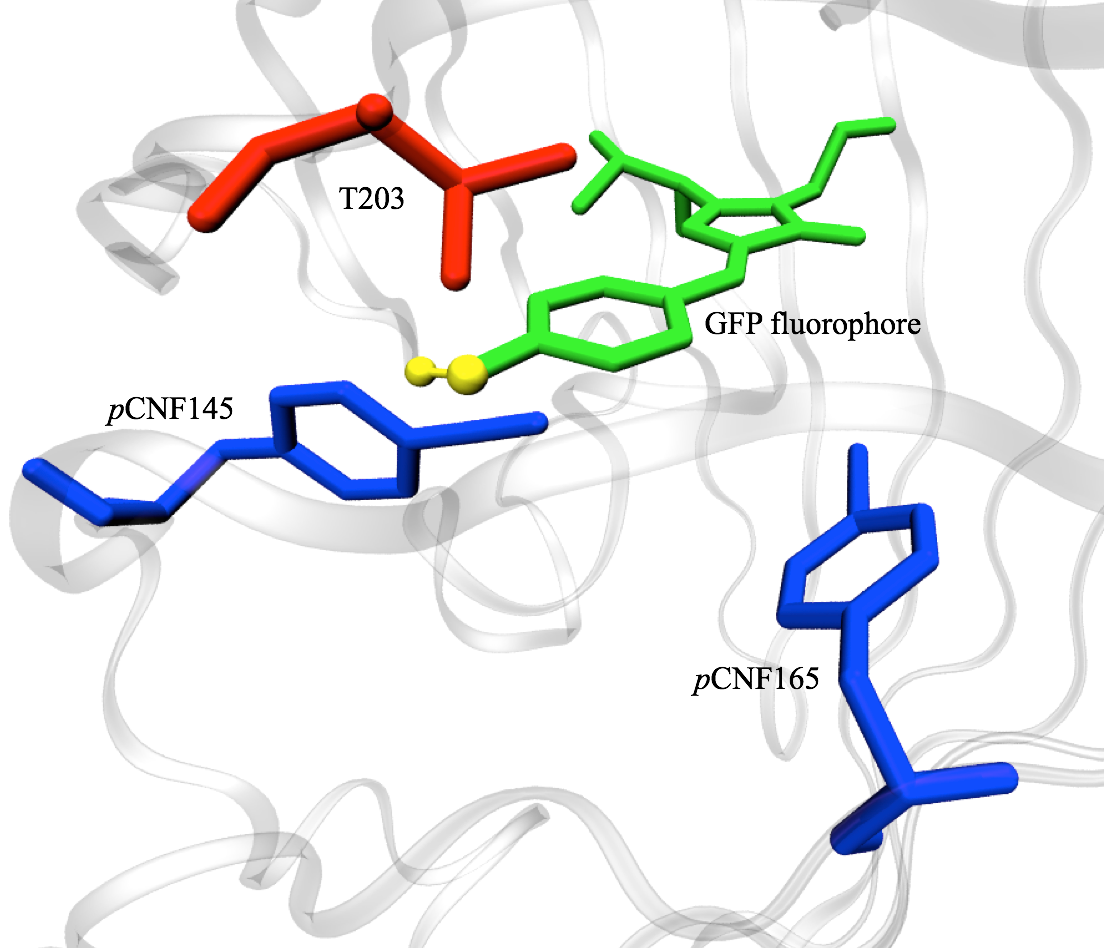
\includegraphics[width=3.25in]{figures-gfp-pKa/system.png}
    \caption{A close-up view of the interior of GFP (gray ribbon) modeled from crystal structure 2b3p. The GFP fluorophore is shown in green with the titratable --OH shown in yellow. \pCNF{} 145 and 165 are shown in blue, and position 203 is shown in red.}
    \label{fig:system}
\end{figure}

Here we report the \pKa{} values of this fluorophore, estimated from the pH-dependent absorption spectra of the GFP fluorophore, as a function of the same mutations. 
To do this, we inserted the unnatural amino acid, \emph{p}-cyanophenylalanine (\pCNF{}), at either position 145 or 165, which are both near the GFP fluorophore, and made a series of mutations to position 203 (Figure \ref{fig:system}). 
We then measured the effect of these mutations on the electrostatic environment in the vicinity of the flourophore both through VSE spectroscopy of the two nitrile probes and \pKa{} and Stark effect measurements of the flourophore itself. 
Our results show that the \pKa{} shifts in response to the amino acid mutations are linearly correlated with the site specific electric field changes, measured from either the vibrational or electronic Stark effect probes. 
This agreement provides confidence that Stark effect shifts and \pKa{} shifts respond similarly to the same electrostatic perturbations. 
This trend was not observed when histidine or cysteine were at position 203, which we hypothesize was due to (1) differences in the hydrogen bonding network around the fluorophore caused by histidine and cysteine at position 203; or (2) the interference of the fluorophore titration by the simultaneous titration of histidine or cysteine at position 203. 
Because of the potential for this experimentally self-consistent model system to be a benchmark for electrostatics models, we also attempted to calculate the \pKa{} values using APBS and molecular dynamics (MD) simulations.
However, even when we included 50 \si{\ns} of protein dynamics, APBS was unable to accurately reproduce the experimental \pKa{} values. 
We predict that a more advanced calculation than one based on a continuum electrostatic treatment of the interior of GFP is likely necessary to accurately predict \pKa{} values inside the unique $\beta$-barrel protein. 
All together, this model system contains a vibrational Stark effect probe, an electronic Stark effect probe, and a \pKa{} probe that all respond similarly to perturbations at position 203. 
In addition to providing confidence in our ability to measure electrostatic effects experimentally, we also believe that these experimental data are an excellent target data set for benchmarking a variety of computational electrostatics models.

%%%%%%%%%%%%%%%%%%%%%%%%%%%%%%%%%%%%%%%%%%%%%%%%%%%%%%%%%%%%%%%%
%%%%%%%%%%%%%%%%%%%%%%%%%%%%%%%%%%%%%%%%%%%%%%%%%%%%%%%%%%%%%%%%
\section{Experimental methods} \label{methods}
%%%%%%%%%%%%%%%%%%%%%%%%%%%%%%%%%%%%%%%%%%%%%%%%%%%%%%%%%%%%%%%%
%%%%%%%%%%%%%%%%%%%%%%%%%%%%%%%%%%%%%%%%%%%%%%%%%%%%%%%%%%%%%%%%

\subsection{Protein Expression and Purification}

A pBAD vector containing the gene for His6-tagged super folder GFP and a pDULE vector coding for an orthogonal tRNA/synthetase pair optimized for \pCNF{} were a generous gift from the Mehl lab \cite{Miyake-Stoner2010}.
Mutations to the pBAD vector at amino acid positions 145, 165, or 203 were made using a Quick Change Mutagenesis kit from Stratagene. 
To make each nitrile-containing GFP mutant, DH10$\beta$ cells were co-transformed with both the pBAD vector (containing the \emph{amber} stop codon at amino acid position 145 or 165, and the proper codon for amino acid 203) and the pDULE vector. 
These co-transformed cells were grown in an autoinduction media as described elsewhere \cite{Hammill2007}.
Mutants without a nitrile probe were purified from DH10$\beta$ cells expressing only the pBAD vector. 
In both cases, the His$_6$-tagged mutants were purified as outlined previously by immobilized metal affinity chromatography, the tags cleaved and separated, and the purified protein used immediately or stored at $-80$ \si{\celsius} \cite{Slocum2016}. 

\subsection{pH Titrations}

Purified GFP mutants were buffer exchanged into a master buffer containing 50 \si{mM} phosphate, 50 mM citrate, and 100 mM NaCl at pH 7.5, and the buffer-exchanged protein was concentrated to $\sim$1 mM using centrifugal filters. 
UV-Vis absorption spectra of the GFP mutants were recorded from pH 5 to 10 on a Biotek Epoch 2 microplate reader between 250-600 nm. 
The plates were prepared by mixing 2 $\mu$L of the concentrated protein with 300 $\mu$L of the master buffer (adjusted to the desired pH with acid or base) into the wells of a UV-transparent 96-well plate. 
For each mutant, at least three pH titrations were carried out.

\subsection{UV-Vis and FTIR Spectroscopy}

For all absorption spectroscopy measurement besides the pH titrations, purified GFP mutants were buffer exchanged into PBS at pH 7.4. 
UV-Vis absorption spectra were collected in a 1 cm quartz cuvette using a Cary 5000 spectrometer with 0.1 nm resolution. 
FTIR absorption spectra of the nitrile-labeled mutants were collected using a Bruker Vertex 70. 
Protein samples concentrated to 1-2 mM were injected between two sapphire windows separated by 125 $\mu$m Teflon spacers. 
Spectra were collected by averaging 250 scans with 0.5 \si{\wn} resolution. 
After subtracting a background spectrum of PBS, the spectra were baseline-corrected and fit to Gaussian functions using an in-house program that has been described previously \cite{Ragain2012}.
All spectra were measured at least three times.   

\subsection{Molecular Dynamics Simulations}

A template protein structure was modeled by homology from the 2b3p crystal structure\cite{Pedelacq2006} using the MODELLER software package \cite{Marti-Renom2000}.
From this template, the 6 different mutations were made to position 203 using the mutagenesis wizard tool in PyMol \cite{DeLano2002}.
For each of these 7 protein systems, the residue at position 145 or 165 was independently mutated to \pCNF{} and minimized using the Avogadro molecular editing package \cite{Hanwell2012}. 
Special care was taken with the titration state of Glu222, which was assigned a neutral state based on indirect crystallographic evidence of the fluorophore hydrogen bonding environment from Remington et al \cite{Elsliger1999}. 
Histidine residues at positions 25, 148 181, 199 and 217 were protonated at the N$_{\delta}$, and histidine residues at positions 77, 81, 139 and 169 was protonated at the N$_{\varepsilon}$, following the simulation protocol by Nifos\'i et al \cite{nifosi2003}.
The histidine at position 231 is not present in either of the two studies cited, and was protonated at the Nε as determined to be most favorable by pdb2gmx. 
Finally, each of these 21 structures was edited to reflect the two different protonation states of the internal GFP chromophore, resulting in 42 different protein systems for the start of molecular dynamics (MD) simulations. 

Parameters for the protonated and deprotonated chromophore were kindly provided by Riccardo Nifos\'i \cite{nifosi2003}.
Point charges for \pCNF{} were derived using the RESP fitting procedure to electrostatic calculations using GAMESS \cite{Bayly1993}.
Bonded parameters for the nitrile group were taken from those previously developed by our group for cyanocysteine \cite{Ragain2012}.
All other bonded parameters were taken by analogy from tyrosine. 
All further minimizations and MD simulations were performed using the Gromacs 5.0.4 molecular dynamics software package \cite{VanDerSpoel2005, Abraham2015} and the Amber03 force field (ffAmber03) \cite{Duan2003, Sorin2005}.
Each of the 42 protein systems was energy minimized in vacuum using steepest descent, and solvated in a 80 \si{\angstrom} dodecahedron box of TIP3P water to ensure that the protein would not interact with itself through the periodic boundary conditions \cite{Jorgensen1983}.
All resulting systems had a net positive charge, which was neutralized with the addition of 5-7 sodium ions, depending on the protein system. 
These solvated systems were energy minimized with heavy atom restraints on the protein, and then were subjected to 100 ps of simulation at constant pressure and 50 ps of simulation at constant volume to equilibrate the solvent, again using heavy atom restraints. 
Production MD was run on each protein system for 50 \si{\ns}, using a time step of 2 fs and stochastic integrator. 
Particle Mesh Ewald electrostatics was implemented with a coulomb cut-off of 8 \si{\angstrom} \cite{Cheatham1995}.
Van der Waals (VDW) interactions were cut off at 8 \si{\angstrom}. 
Snapshots were recorded every 4 ps during the simulations.  

\subsection{Electrostatic Free Energy Calculations in APBS}

At every 500 ps of each simulation, molecular structure, including a 5 \si{\angstrom} sphere of explicit waters as discussed below, was extracted using the Gromacs utilities select and trjconv. 
Charges and VDW radii were assigned to the molecular structures using the pdb2pqr utility provided with the APBS v1.4 software package \cite{Dolinsky2007}.
The GFP chromophore and \pCNF{} charges were taken in accordance with their simulation point charges, and VDW radii were assigned by analogy to other atom types.

To assess the free energy of protein-solvation, three electrostatic free energy calculations were performed using APBS on the protein-solvent structure, the protein-solvent structure with charges on the chromophore removed, and an isolated chromophore structure. 
In each of these calculations, the same grid spacing was used in accordance with the default pdb2pqr suggestion for a system of this size. 
The solvent region was assigned a dielectric constant of 78.54 and the protein region was assigned a dielectric constant of 6. 
For free energy calculations on the crystal structures, the protein region and any crystallized water molecules were assigned a dielectric constant of 20 instead as the conformational flexibility of the protein was not explicitly simulated.

%%%%%%%%%%%%%%%%%%%%%%%%%%%%%%%%%%%%%%%%%%%%%%%%%%%%%%%%%%%%%%%%
%%%%%%%%%%%%%%%%%%%%%%%%%%%%%%%%%%%%%%%%%%%%%%%%%%%%%%%%%%%%%%%%
\section{Results and Discussion} \label{results}
%%%%%%%%%%%%%%%%%%%%%%%%%%%%%%%%%%%%%%%%%%%%%%%%%%%%%%%%%%%%%%%%
%%%%%%%%%%%%%%%%%%%%%%%%%%%%%%%%%%%%%%%%%%%%%%%%%%%%%%%%%%%%%%%%

\subsection{\pKa{} Measurements}

To compare the ability of \pKa{} shifts and Stark effect shifts to report on changes in electrostatic environment in a protein, we mutated the wild type T203 (where T represents the one letter code of threonine and 203 is the amino acid position in the primary sequence) of superfolder GFP to S, N, H, C, F, and Y and inserted a \pCNF{} residue at either position 145 or 165 (Figure \ref{fig:system}). 
To estimate the equilibrium between the neutral and ionized fluorophore, we measured the pH dependence of the visible absorption of the fluorophore over a range of pH 5-10.  
Figure \ref{fig:abs_titrations} shows the pH-dependent visible absorption spectra of a representative GFP mutant, S203 (Figure \ref{fig:abs_titrations}A), and the resulting titration curve (Figure \ref{fig:abs_titrations}B), from which the \pKa{} values were determined. 
As expected, the fluorophore population shifted from mostly protonated (A state) at low pH to mostly de-protonated (B state) at high pH.
The presence of a clean isosbestic point indicated that there were only two states participating in the equilibrium.
Plotting the maximum absorbance of both the A and the B states as a function of the solution pH resulted in two curves which could be fit to a single sigmoidal function and used to find the inflection point.
The curve fitting application of Matlab R2016a was used to fit all titration curves to a sigmoidal function of the form shown in Equation \ref{eq:sigmoid},
\begin{equation}
    \text{Abs}(\pH) = \frac{a}{b+e^{c\cdot\pH}}+d
    \label{eq:sigmoid}
\end{equation}
where Abs(pH) is the maximum absorbance of either the A or B state at a given pH, $a$ is the maximum value of Abs, $b$ defines the offset of the function from pH = 0, $c$ defines the pitch of the sigmoid, and $d$ is the minimum value of Abs \cite{Matlab2016}.
The inflection point of the resulting fit was taken to be the \pKa{} for that mutant.
The titration curves for each of the 21 mutant constructs is shown in Supplemental Information, Figure S1.
With the exception of the few cases where the A state titration could not be fit (Y203, H203, and H203 with \pCNF{} 165) in Figure S1, titrations of both the A and B states gave \pKa{} values that were within experimental error of each other, < 0.08 \pKa{} units.
In the cases where only one titration could be fit to a sigmoidal curve, the \pKa{} was estimated directly from that titration.
The fact that 39 of the 42 titrations in Figure S1 gave data that could be well described by a single site titration model suggests that any coupling of the fluorophore titration to other nearby titratable residues is negligible. 

\begin{figure}
    \center
    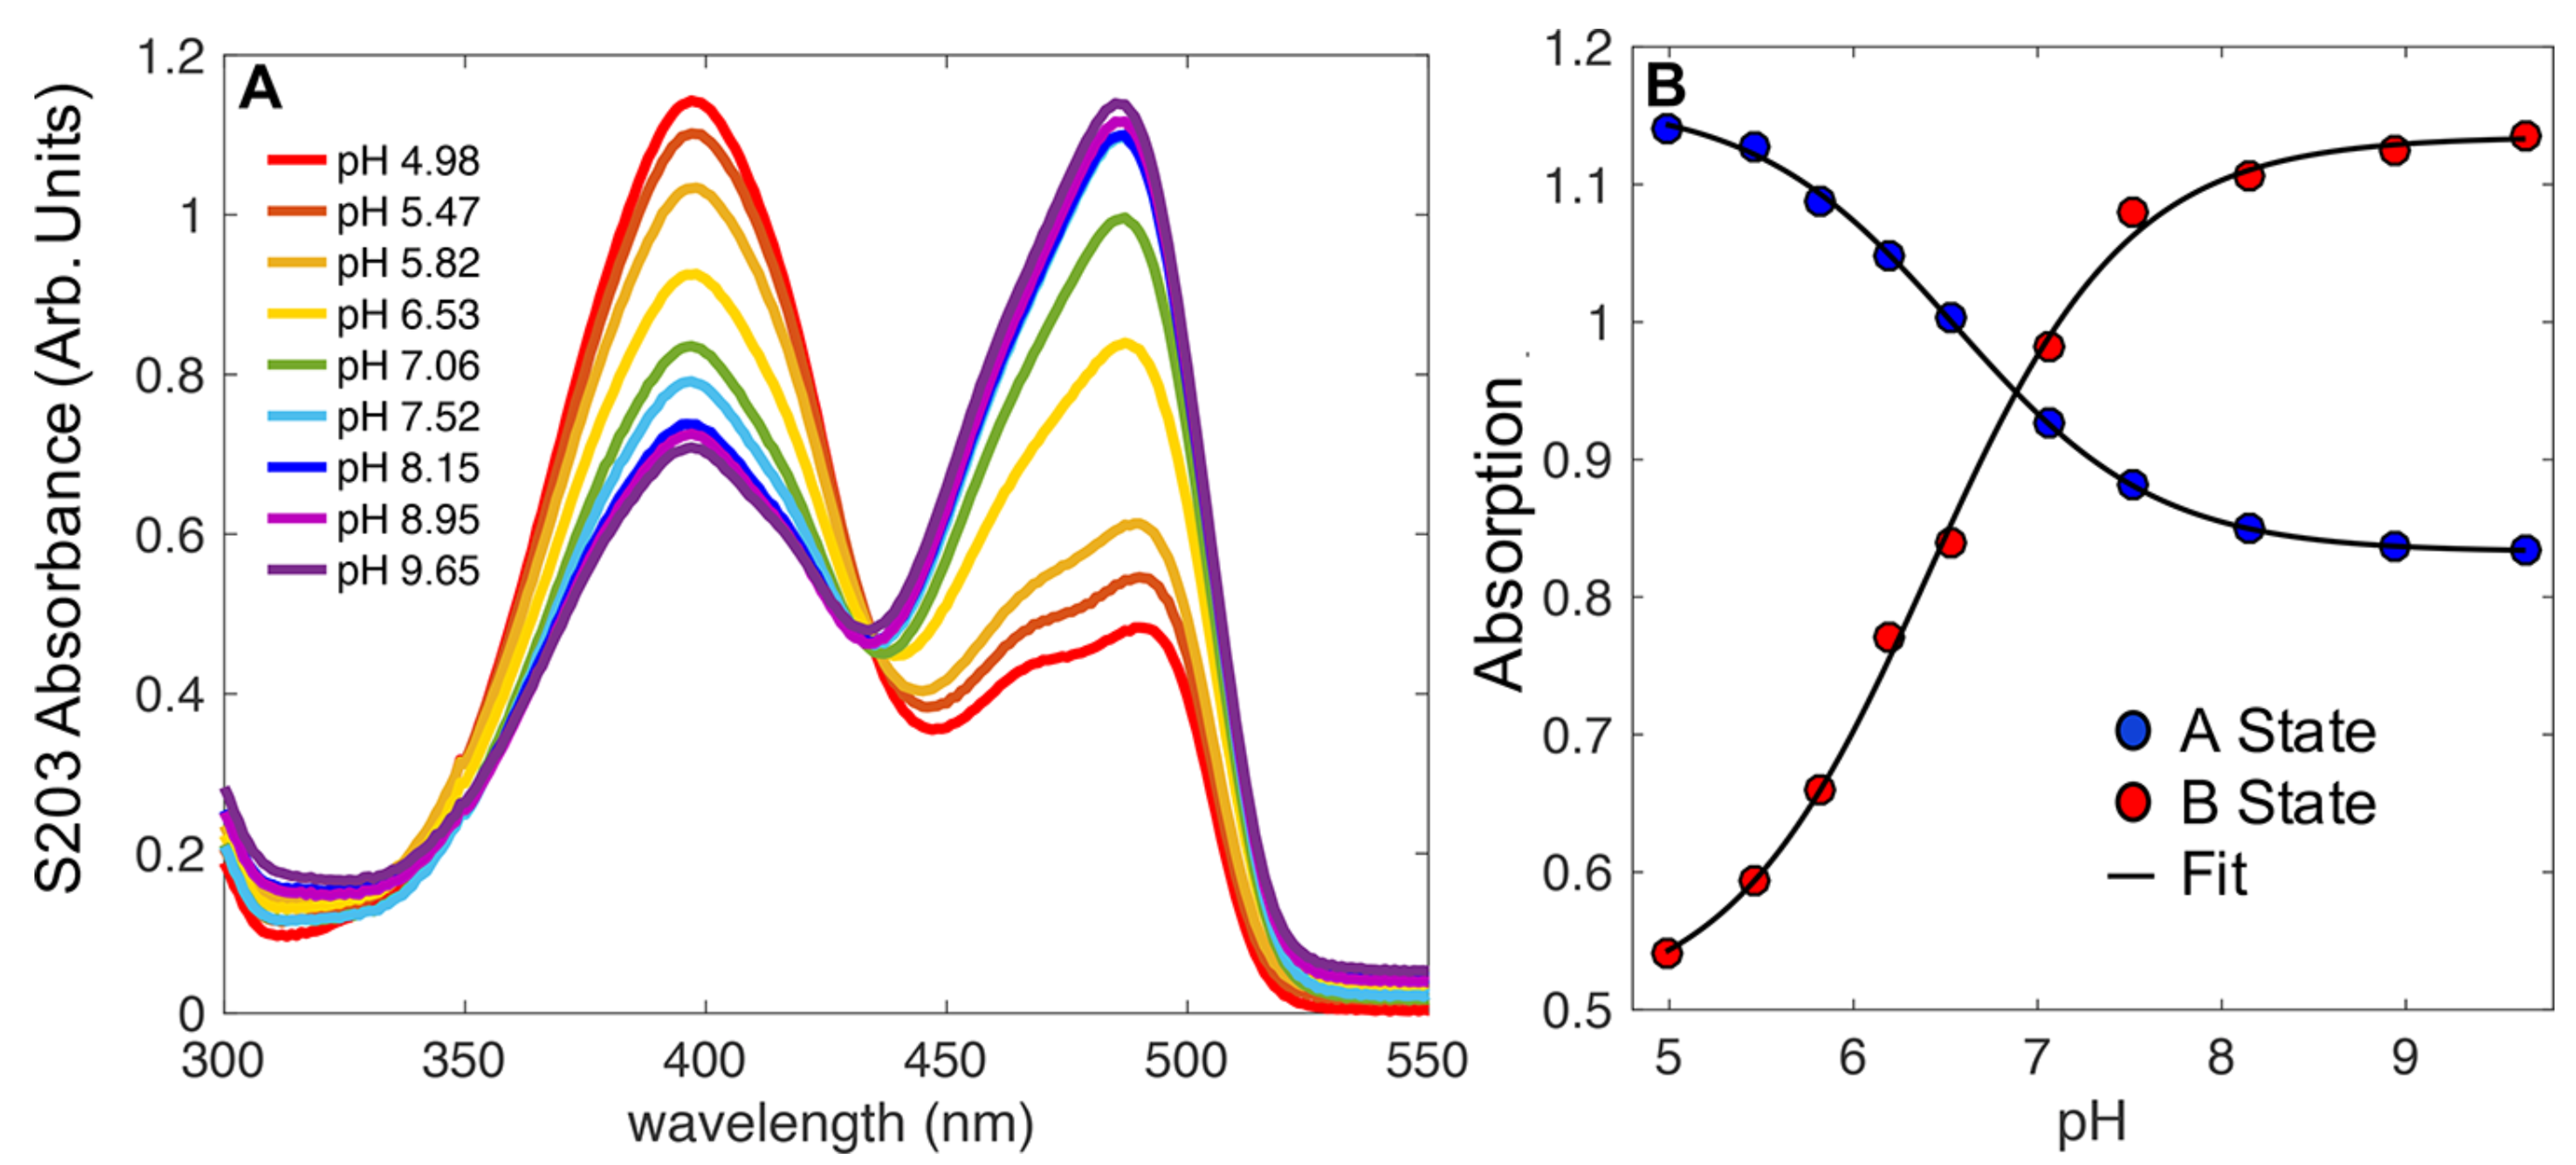
\includegraphics[width=0.8\linewidth]{figures-gfp-pKa/absorption_titrations.png}
    \caption{A representative titration of the GFP fluorophore. Panel A shows the visible absorption spectra of the fluorophore of S203 over a range of pH values given by the color code. Panel B shows the maximum absorption of the A state (blue) and the B state (red) of the S203 spectra from panel A, plotted against the solution pH. The solid lines are sigmoidal fits which are used to estimate the \pKa{}.}
    \label{fig:abs_titrations}
\end{figure}

Table \ref{tbl:pKas} shows the \pKa{} values obtained for all 21 of the mutant constructs.
Overall, we measured a range of \pKa{} values from 6.28-8.04, which is typical for GFP mutants containing the TYG fluorophore.
Previous studies have suggested that two dominating contributions to GFP fluorophore \pKa{} values are (1) specific hydrogen bonding to or from the fluorophore phenolate (or phenol), determined by the local hydrogen bonding network of water and protein residues around the fluorophore; and (2) aromatic interactions with the fluorophore from nearby side chains that tend to stabilize the neutral form of the fluorophore.54,65
Here, the measured \pKa{} values tended to increase as we placed aromatic residues at position 203, and the lowest \pKa{} values were measured for the small, polar residues at position 203.
This suggests that aromatic interactions between the fluorophore and Y and F at position 203 are responsible for the elevated \pKa{} values we have measured here, and that the hydrogen bonding environment around the fluorophore might play a larger role in the \pKa{} values for the other position 203 mutants. 

\begin{table}
    \begin{center}
    \caption{A Summary of the Measured pKa Values for All GFP Mutants$^a$}
    \begin{tabular}{c|ccc}
        \toprule
        \rowcolor{lgray}
        position 203 & WT & \pCNF{} 145 & \pCNF{} 165 \\

        \cmidrule(r){1-1}\cmidrule(l){2-4}
        T$^b$ &   $ 6.70 \pm 0.07 $  &  $ 6.63 \pm 0.04 $ &  $ 7.17 \pm 0.03 $  \\
        F     &   $ 7.50 \pm 0.03 $  &  $ 7.20 \pm 0.04 $ &  $ 7.51 \pm 0.05 $  \\
        C     &   $ 6.85 \pm 0.05 $  &  $ 7.86 \pm 0.04 $ &  $ 7.65 \pm 0.04 $  \\
        H     &   $ 6.54 \pm 0.03 $  &  $ 6.28 \pm 0.05 $ &  $ 6.77 \pm 0.05 $  \\ 
        N     &   $ 7.11 \pm 0.08 $  &  $ 7.22 \pm 0.04 $ &  $ 7.42 \pm 0.06 $  \\ 
        S     &   $ 6.48 \pm 0.07 $  &  $ 6.88 \pm 0.07 $ &  $ 6.73 \pm 0.05 $  \\ 
        Y     &   $ 7.95 \pm 0.04 $  &  $ 7.95 \pm 0.04 $ &  $ 7.95 \pm 0.03 $  \\ 

        \bottomrule
    \end{tabular}
    \end{center}

    $^a$Columns are the different nitrile locations: WT (No nitrile), \pCNF{} at position 145, and \pCNF{} at position 165. The rows designate the different amino acid side chains at position 203 based on the one-letter codes in the first column. 
    $^b$The identity of position 203 in the wild-type protein is T.
    \label{tbl:pKas}
\end{table}

\subsection{Vibrational and Electronic Absorption Measurements}

To further investigate these interactions and their importance in determining fluorophore \pKa{}, we compared measured \pKa{} changes to the orthogonal site-specific electric field measurements obtained through spectroscopic Stark effect measurements using both the GFP fluorophore and the biosynthetically incorporated \pCNF{} residues.
We measured the absorption spectra of the GFP fluorophore and the inserted \pCNF{} probes at pH 7.4.
Figure \ref{fig:abs_spectra} shows representative spectra of all variants investigated.
Figures \ref{fig:abs_spectra}A, \ref{fig:abs_spectra}B, and \ref{fig:abs_spectra}C show the fluorophore absorption as a function of the position 203 mutations when there is no \pCNF{}, \pCNF{} at position 145, and \pCNF{} at position 165, respectively.
All visible spectra showed the same general shape, with two major features which have been well characterized as being due to the neutral (A state: $\sim$400 \si{\nm}) and ionized (B state: $\sim$500 \si{\nm}) forms of the fluorophore.
There were two distinct types of changes in these spectra that resulted from the position 203 mutations.
First, changes in the relative intensities of the two major peaks indicated that the equilibrium between neutral and ionized fluorophore changed (for example, Y and T in Figure \ref{fig:abs_spectra}A, which show different ratios of absorbance between the A and B states).
Second, the energies of maximum absorption of both the A and B state changed in response to the position 203 mutations.
The B state absorption energies, which have been shown to be well described by Equation \ref{eq:stark}, with $\Delta\vec{\mu}$ = 117.5 \si{\wn}/(MV/cm)44 for absorption of the electronic fluorophore, will be used in the following sections to calculate electric field changes experienced by the fluorophore.
However, the A state absorption energies, which still changed as a function of the mutations, are not well described by the linear Stark effect and cannot be straightforwardly related to electric field changes.44
Figure \ref{fig:abs_spectra}D shows the representative \pCNF{} absorption spectra of \pCNF{} 145 (solid) and 165 (dashed).
With the exception of the mutant containing C203 and \pCNF{} 145 (Figure \ref{fig:abs_spectra}D, solid yellow line), all of these spectra could be well described by a single Gaussian whose center frequencies spanned a range of approximately 2 \si{\wn} across all mutants of position 203.
As we previously reported, the \pCNF{} 145 spectra were quite narrow ($\sim$5-6 \si{\wn} FWHM, except C203) and the \pCNF{} 165 spectra were somewhat more broadened ($\sim$8-9 \si{\wn}), suggesting that the nitriles at position 165 experience a more heterogeneous environment than the nitriles at position 145.
In addition to this, the \pCNF{} 145 and 165 spectra were separated from each other in energy by $\sim$10 \si{\wn} depending on the identity of the side chain of position 203.
Altogether, these spectra suggest that the local environment around position 145 is quite different than that of position 165, despite their proximity to one another (Figure \ref{fig:system}).
This is likely a reflection of the environmental complexity of the interior of GFP, which could be manifested in different hydrogen bonding environments or local conformational fluctuations of the nitriles, and will be discussed in more detail below.

\begin{figure}
    \center
    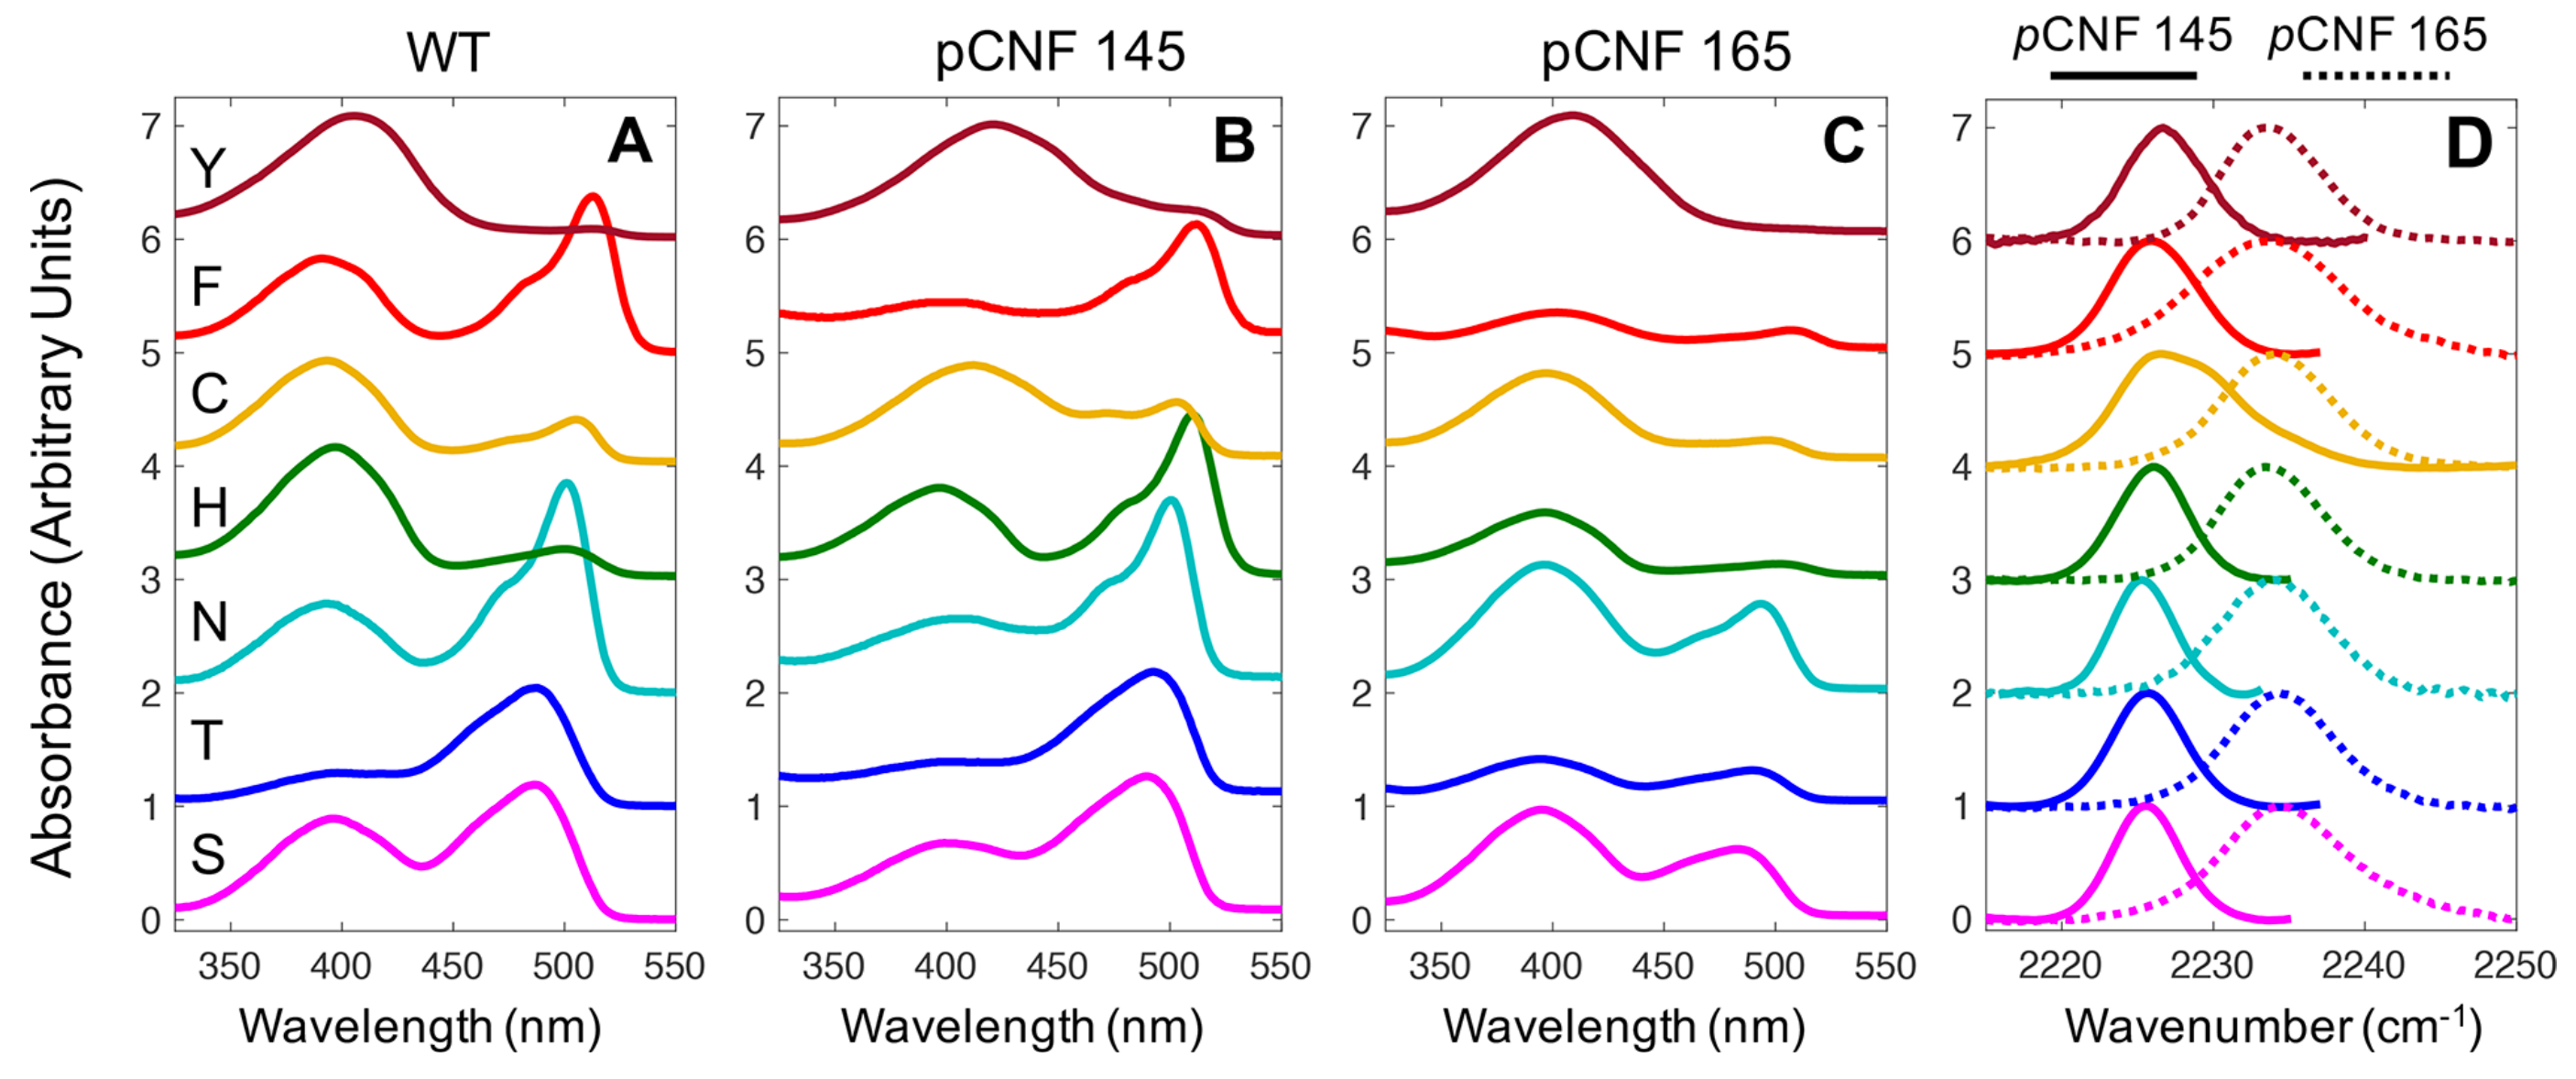
\includegraphics[width=6.0in]{figures-gfp-pKa/abs_spectra.png}
    \caption{Representative absorption spectra for all GFP mutants recorded at pH 7.4. Panels A, B, and C show the visible absorption of the GFP fluorophore normalized to the absorbance at 280 nm for proteins that have no nitrile probe (A), \pCNF{} at position 145 (B), and \pCNF{} at position 165 (C). Different colors represent the different amino acid side chains at position 203 based on the one-letter code in panel A. Panel D shows the FTIR absorption of the \pCNF{} residue at either position 145 (solid) or 165 (dashed) with the same colors to denote different amino acids at position 203. All spectra have been offset on the y-axis for clarity.}
    \label{fig:abs_spectra}
\end{figure}

\subsection{Comparing \pKa{} Shifts to Electronic Stark Effect Shifts}

To compare the changes in fluorophore \pKa{} to changes in electric field experienced by the fluorophore, we plotted the \pKa{} changes for all unique pairs of the seven mutants against the corresponding changes in electric field experienced by the fluorophore (calculated from Equation \ref{eq:stark}) in Figure \ref{fig:pKa_vs_stark}.
The data in Figures \ref{fig:pKa_vs_stark}A-C were generated from GFP constructs that contained no nitrile probe (Figure \ref{fig:pKa_vs_stark}A), \pCNF{} at position 145 (Figure \ref{fig:pKa_vs_stark}B), or \pCNF{} at position 165 (Figure \ref{fig:pKa_vs_stark}C).
In this case, the seven individual \pKa{} values and deprotonated fluorophore absorption energies from the position 203 mutants gave rise to 21 distinct \pKa{} shifts and absorption energy changes.
We used these absorption energy changes and the known Stark tuning rate of the deprotonated GFP fluorophore to calculate the electric field changes experienced by the fluorophore from Equation \ref{eq:stark}.
For all of these comparisons, we observed a strong linear correlation between the fluorophore \pKa{} shifts and corresponding Stark effect shifts due to the position 203 mutations, which suggests that these two orthogonal measurements responded similarly to the same electrostatic perturbation.
More specifically, the mutations that caused large, positive electric field changes in the direction of the fluorophore difference dipole moment tended to cause concurrent increases in the fluorophore \pKa{} (to favor the neutral versus negatively charged form).
Conversely, mutations that caused large electric field changes anti-parallel to the difference dipole moment of the fluorophore tended to push the equilibrium toward the negative form of the fluorophore.
Furthermore, responses to electrostatic perturbations followed previously observed patterns based on the chemical identity of the mutant residue.
In Figure \ref{fig:pKa_vs_stark}, the different colors represent the type of mutation that was made at position 203 based on the key in Figure \ref{fig:pKa_vs_stark}A.
For instance, the magenta points represent mutations involving the replacement of an -OH side chain (T or S) with an aromatic side chain (F or Y), similar to the mutation made in yellow fluorescent protein.65.
We previously observed that mutations of this nature, and their opposites (red in Figure \ref{fig:pKa_vs_stark}), are responsible for the largest changes in electric field, measured spectroscopically.
In this work, we see that these mutations also cause the largest shifts in \pKa{}.
Additionally, we saw that conservative mutations (e.g. S to T or F to Y; black in Figure \ref{fig:pKa_vs_stark}) tended to cause the smallest changes in both \pKa{} and electric field experienced by the fluorophore.
The observation that the Stark effect shifts and \pKa{} shifts of the fluorophore are not only linearly correlated, but also respond similarly to the same types of mutations (denoted by the colors in Figure \ref{fig:pKa_vs_stark}), gives us confidence that these two orthogonal probes of electrostatic perturbation are indeed reporting on a common electrostatic effect.

\begin{figure}
    \center
    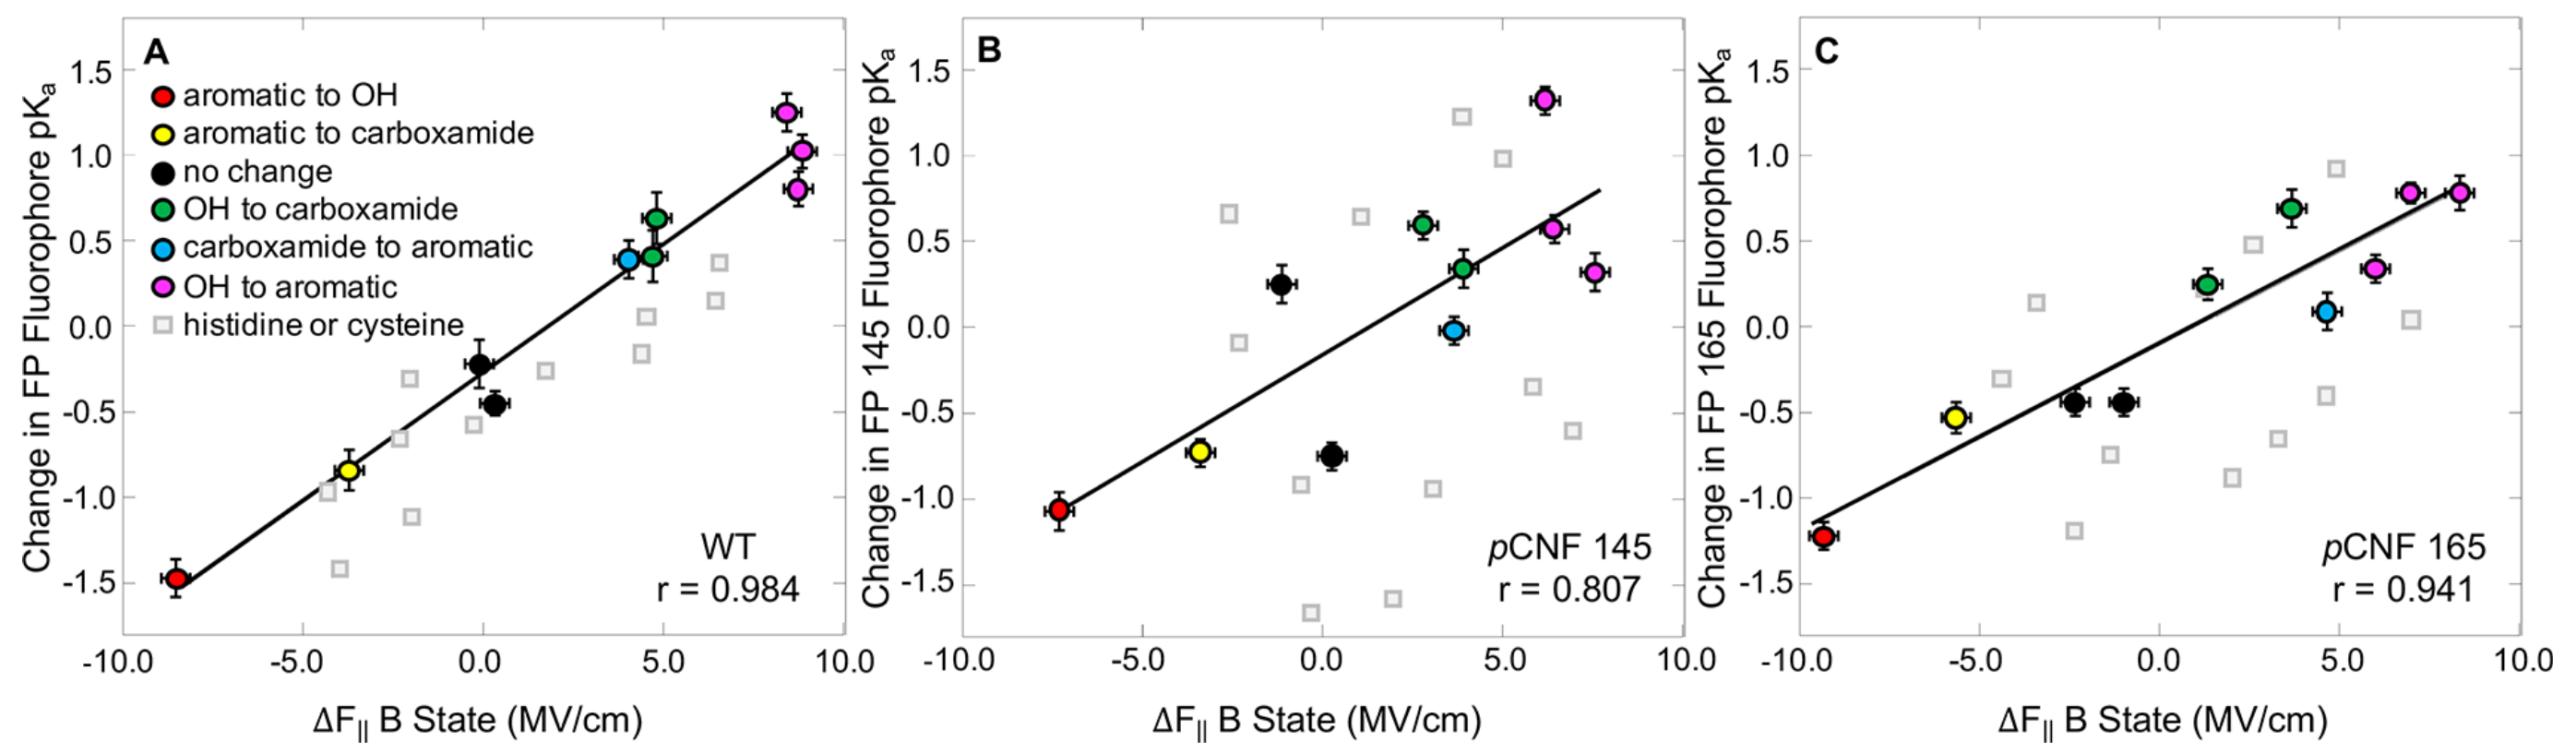
\includegraphics[width=6.0in]{figures-gfp-pKa/pKa_vs_elec_stark.png}
    \caption{Changes in the measured fluorophore pKa plotted against changes in the electric field experienced by the B state of the fluorophore for GFP mutants with (A) no nitrile probe present, (B) \pCNF{} at position 145, and (C) \pCNF{} at position 165. Different colors represent the type of mutation that was made to position 203 based on the key in panel A. Gray squares represent position 203 mutations that involved changes to or from histidine or cysteine and are omitted from the best fit lines and correlation constants. Error bars on the x-axis represent uncertainty in the published Stark tuning rate of the deprotonated GFP fluorophore. Error bars on the y-axis represent standard deviations in the inflection points of at least three \pKa{} titration curves.}
    \label{fig:pKa_vs_stark}
\end{figure}

In Figure \ref{fig:pKa_vs_stark}, however, there are clear deviations from this linear correlation.
In displaying the data in this manner, it is apparent that, with the exception of the proteins with no \pCNF{} probe (4A), mutations to or from histidine or cysteine (gray squares in Figure \ref{fig:pKa_vs_stark}) caused \pKa{} changes that were in poor agreement with the corresponding Stark effect shifts of the GFP fluorophore.
Of the seven side chains we placed at position 203, H and C are clearly different from the rest because they can be titrated near physiological pH (the \pKa{} values of H and C side chains in water are 6.0 and 8.1, respectively).
It is reasonable to suspect that the presence of a second titration site (H or C at position 203) might complicate the straightforward analysis of the GFP fluorophore equilibrium and contribute to the weakening of the correlations shown in Figures \ref{fig:pKa_vs_stark}B and \ref{fig:pKa_vs_stark}C.
However, the fact that the disagreement between electronic Stark effects and \pKa{} shifts for these mutations is only apparent when either nitrile probe is present suggests that the presence of \pCNF{} is the cause of the disagreement.
Because of the likely role of hydrogen bonding to the fluorophore in determining its \pKa{}, and the ability of the nitrile group to accept a hydrogen bond, we think it is likely that \pCNF{} at either of these locations could potentially disrupt the hydrogen bonding network in the interior of GFP, which could in turn perturb the native \pKa{} values.
Further studies are underway to investigate changes in the hydrogen bonding network near the GFP fluorophore induced by the insertion of \pCNF{} residues at positions 145 and 165 to test this hypothesis.
In the sections that follow, we address the electrostatic perturbations induced by the nitrile probes and how they affect our ability to interpret the measured vibrational energies in a meaningful way.

\subsection{\pKa{} Perturbations Due to Nitrile Probes}

One of the principal criticisms of using nitrile vibrational probes in biological molecules is that the inclusion of the nitrile itself, an oscillator with a large ground state dipole moment and hydrogen bond accepting ability, will inherently perturb the biomolecule, and is not a reliably benign reporter of the molecular environment of interest.66
The observation discussed above, that mutations to C or H deviate from the otherwise strong correlation between \pKa{} and Stark effect shift when a nitrile probe is present, may indeed be evidence of this effect.
To investigate this, we examined the ability of the nitrile probes to perturb the fluorophore \pKa{} values, relative to the values with no nitrile probe present.
This is shown in Figure \ref{fig:pKa_sidechain}, where the change in fluorophore \pKa{} of all position 203 mutants (indicated by the one letter code on the x-axis) is plotted as a function of a nitrile located at either position 145 (black) or 165 (red).
For most of the mutants, we saw that the insertion of a \pCNF{} residue at either position induced a \pKa{} change of at least $\pm$ 0.2 pH units, which represents a significant electrostatic perturbation due to the nitrile probe.
Because the nitrile moiety can accept a hydrogen bond from either water or a nearby amino acid residue, inserting \pCNF{} into the $\beta$-barrel of GFP has the potential to disrupt the hydrogen bonding network around the fluorophore, which could explain the significant \pKa{} changes in Figure \ref{fig:pKa_sidechain}.
C203 mutants with either nitrile probe clearly exhibit the largest observed \pKa{} shifts, up to 1 pH unit, which further supports our decision to remove C203 from the trends in Figure \ref{fig:pKa_vs_stark}.
This highlights the care that should be taken when using nitriles as electrostatic probes.

\begin{figure}
    \center
    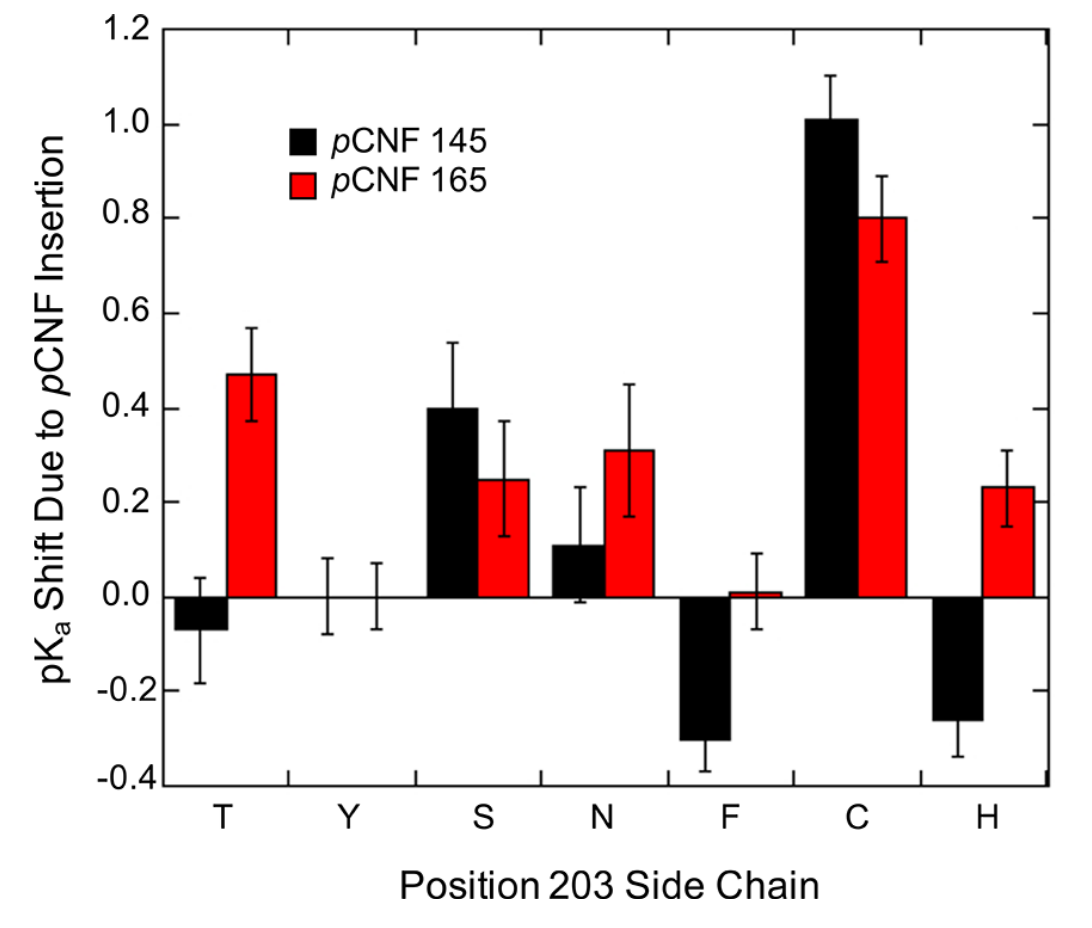
\includegraphics[width=3.25in]{figures-gfp-pKa/pKa_by_side_chain.png}
    \label{fig:pKa_sidechain}
    \caption{\pKa{} shift of the GFP fluorophore caused by the insertion of \pCNF{} at position 145 (black) or 165 (red) for each amino acid at position 203 (one letter code on the x-axis). Error bars represent the standard deviation of at least three titrations.}
\end{figure}

In contrast, the \pCNF{} residues appear to perturb the chromophore environment the least when Y or F is at position 203.
Previous work has suggested that aromatic van der Waals interactions between the residue at position 203 and the fluorophore, as well as specific hydrogen bonding to and from the fluorophore, are the dominating contributions to GFP fluorophore \pKa{}.54
As such, we think that the mutants containing Y or F at position 203 have \pKa{} values that are dominated by aromatic interactions, and thus should be less sensitive to subtle changes in the surrounding hydrogen bonding network.
Therefore, with the view that the perturbations shown in Figure \ref{fig:pKa_sidechain} were caused by differences in the hydrogen bonding network around the fluorophore due to the \pCNF{} residues, it makes sense that the smallest perturbations were observed for mutants with Y or F at position 203.
This is further supported by the elevated \pKa{} values we measured for the Y203 and F203 mutants ($\sim$7.5-8.0; Table \ref{tbl:pKas}), which suggest that aromatic interactions between Y203 or F203 and the fluorophore work to stabilize the protonated form of the fluorophore.
Interestingly, with the exception of F203 and H203 mutants containing \pCNF{} 145, the insertion of the nitrile probe either caused no measurable \pKa{} change or caused a shift to higher \pKa{} values (in favor of the neutral fluorophore).
While it is difficult to ascribe this general increase in fluorophore \pKa{} to any specific interactions, it may be the result of favorable aromatic interactions between the fluorophore and the nearby \pCNF{} 145 or 165.
Additionally, the inserted nitrile probes might disrupt the hydrogen bonding environment around the fluorophore in a systematic way that tends to favor the neutral fluorophore. 

\subsection{Comparing \pKa{} Shifts to Vibrational Stark Effect Shifts}

As we have observed before, \pCNF{} at positions 145 and 165 can perturb the native environment around the GFP fluorophore.
However, regardless of the mechanism by which these nitrile probes shift the \pKa{} of the GFP fluorophore, our primary interest is in relating changes in their measured vibrational energies to changes in electric field via Equation \ref{eq:stark}.
We previously observed that, even though \pCNF{} introduced large electric field perturbations into GFP, changes in the nitrile absorption energy could still be related to electric field changes that were verified by an independent electric field reporter.43
We hypothesized that a similar effect might happen here, where the observed \pKa{} perturbations due to \pCNF{} 145 and 165 might be cancelled out such that differences in \pKa{} can still be correlated to VSE shifts of the nitriles.
To investigate this possibility, we directly compared the nitrile Stark effect shifts to the \pKa{} shifts of the fluorophore, caused by the mutations at position 203.
Figure \ref{fig:pKa_vs_cnf} shows the fluorophore \pKa{} changes due to all unique pairs of the seven position 203 mutants plotted against the corresponding electric field changes projected onto either \pCNF{} 145 (Figure \ref{fig:pKa_vs_cnf}A) or 165 (Figure \ref{fig:pKa_vs_cnf}B) calculated from Equation \ref{eq:stark} using the nitrile absorption energies as determined from Figure \ref{fig:abs_spectra}D.
Similar to the data shown in Figure \ref{fig:pKa_vs_stark}, we observed a linear correlation between the \pKa{} shifts and the corresponding electric field changes experienced by the \pCNF{} residues, which further strengthens our confidence in the ability of these two orthogonal measurements to report on the same electrostatic perturbations.
Additionally, based on the color key in Figure \ref{fig:pKa_vs_cnf}B, we saw that the same trends in position 203 side chain that were observed from the fluorophore Stark effect response (Figure \ref{fig:pKa_vs_stark}) were observed in the response of these nitrile probes.
The trend lines in Figure \ref{fig:pKa_vs_cnf}A and \ref{fig:pKa_vs_cnf}B have slopes that differ in both sign and magnitude, which highlights the geometric dependence of the vibrational Stark effects shifts (dot product in Equation \ref{eq:stark}).
Because \pCNF{} 145 and 165 are spatially removed from each other and oriented in different directions (Figure \ref{fig:system}), we should not expect the projection of an electric field change on to their respective bond axes to result in the same changes in energy.

\begin{figure}
    \center
    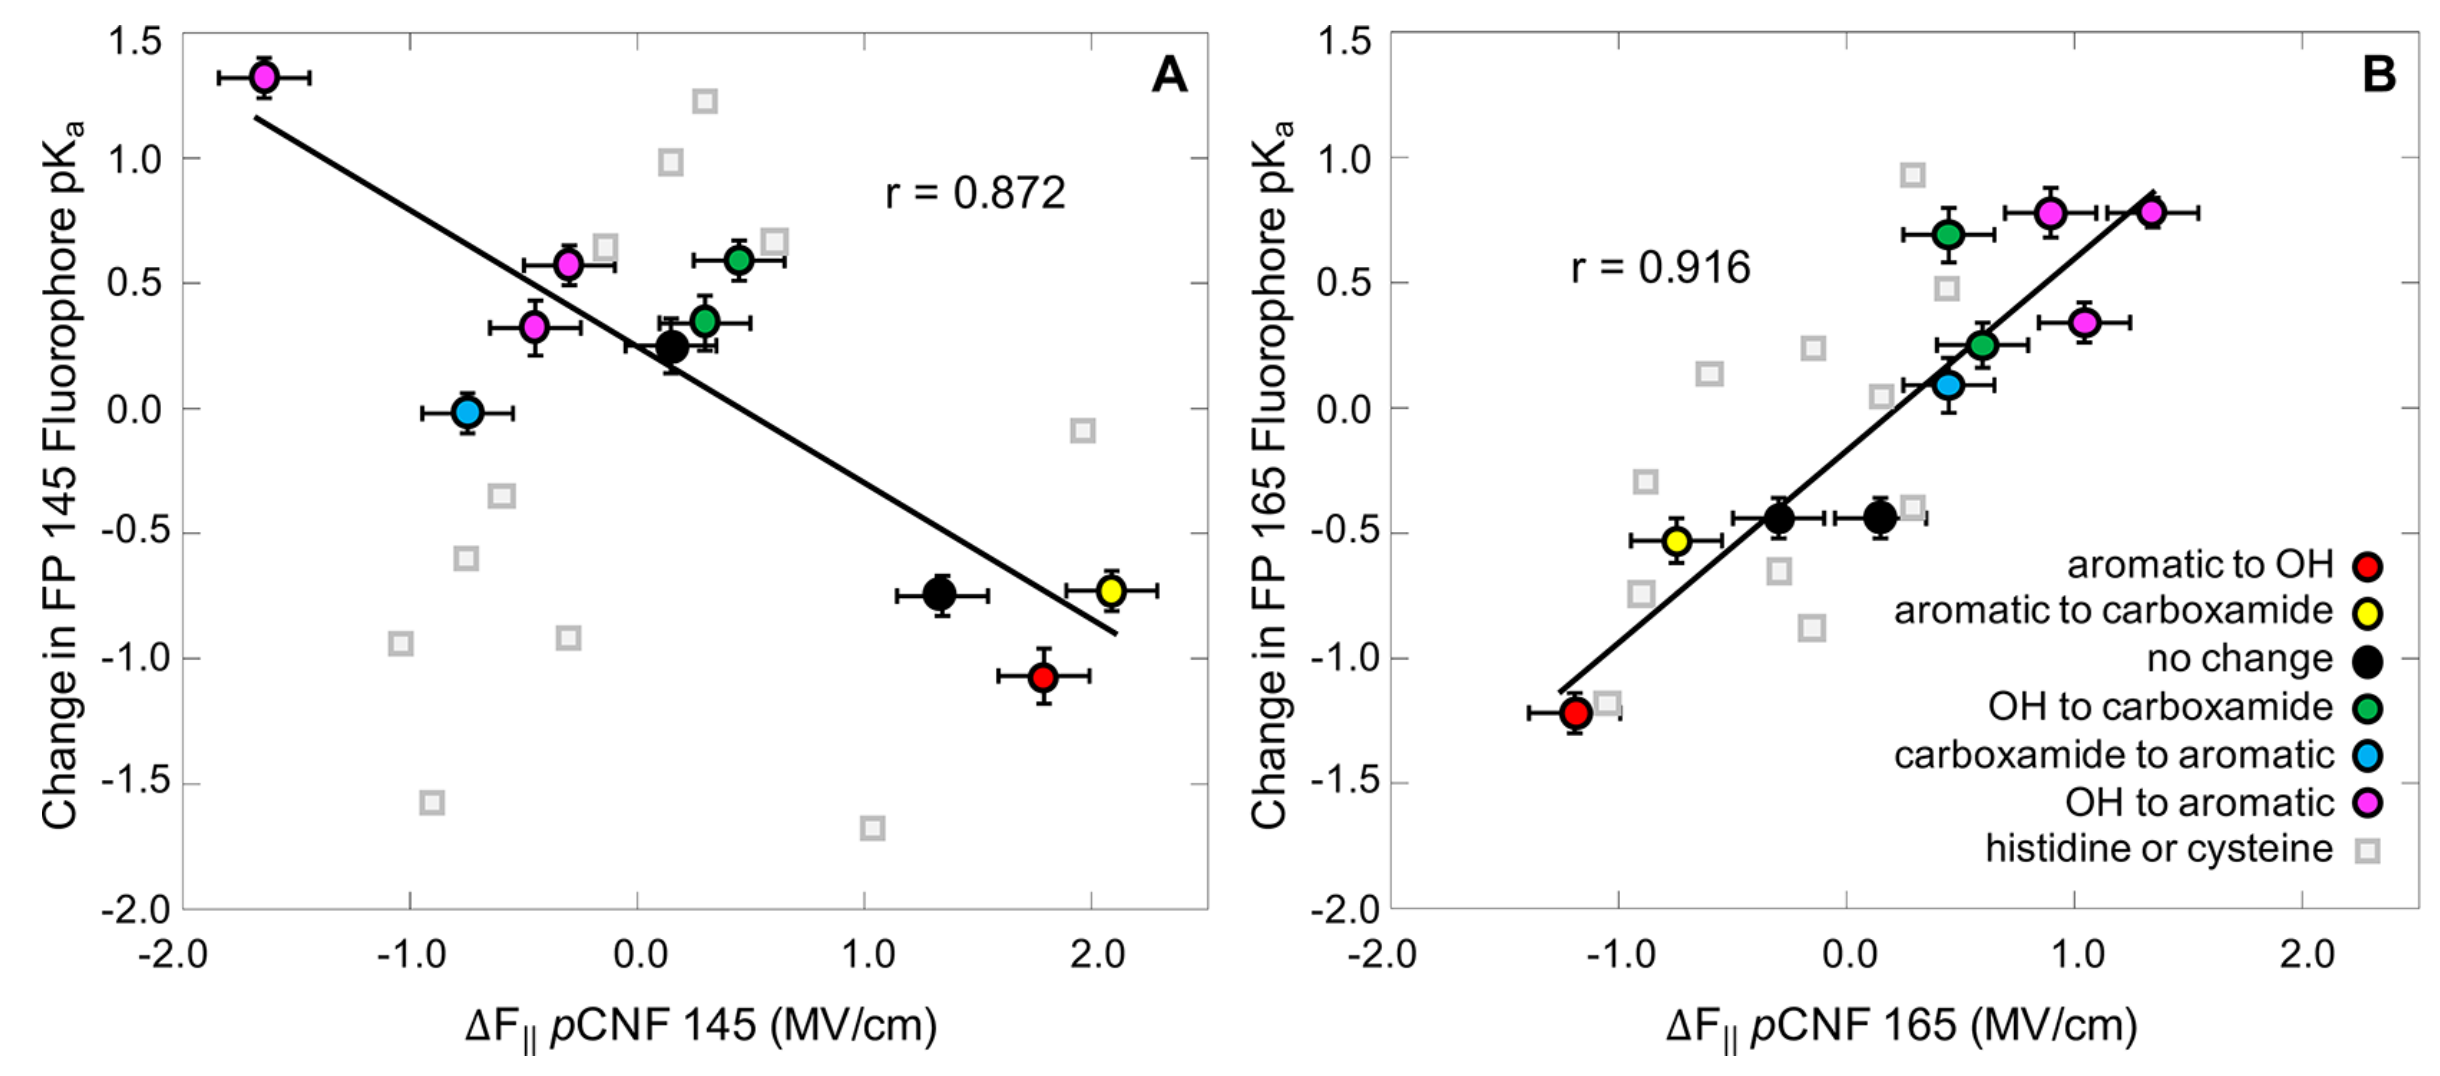
\includegraphics[width=6.0in]{figures-gfp-pKa/pKa_vs_cnf.png}
    \label{fig:pKa_vs_cnf}
    \caption{Changes in the fluorophore \pKa{} plotted against the electric field changes measured from \pCNF{} 145 (A) and 165 (B) for all unique pairs of the seven position 203 mutants. Colors represent the type of mutation made to position 203 based on the key in panel B. Gray squares represent position 203 mutations that involved changes to or from histidine or cysteine and are omitted from the best fit lines and correlation constants. Error bars on the x-axis represent uncertainty in the published Stark tuning rate of \pCNF{}. Error bars on the y-axis represent standard deviations in the inflection points of at least three titration curves.}
\end{figure}

The observed linear correlation between VSE shifts of these inserted nitriles and the corresponding fluorophore \pKa{} shifts is remarkable.
In the previous section, we showed that \pCNF{} 145 and 165 can significantly perturb the fluorophore \pKa{} values (Figure \ref{fig:pKa_sidechain}), and yet the changes in \pKa{} are still well correlated to the measured VSE shifts (Figure \ref{fig:pKa_vs_cnf}).
This is similar to what we have previously reported, where \pCNF{} residues at these positions in GFP cause a significant electrostatic perturbation to the fluorophore, but do not affect GFP's intrinsic fluorescence sensitivity to the position 203 mutations.43
The perturbations caused by \pCNF{} residues in GFP appear to be systematic, such that the comparison between two states allows any perturbations caused by the experiment itself to be cancelled and the resulting energy difference to be interpreted in a meaningful way.
However, again it is clear that mutations to or from cysteine and histidine caused a weakening in the correlation between the \pKa{} shifts and the electric fields measured from each \pCNF{} residue, although the effect is worse for \pCNF{} 145 than it is for \pCNF{} 165. 

Because of our assertion that the \pKa{} and Stark effect shifts represent orthogonal responses to the same electrostatic perturbations, we wanted to explore the idea that the nitrile frequencies might simply shift as a result of differences in the concentration of protonated and deprotonated fluorophores.
For instance, if the A and B states of the fluorophore exert different electric fields onto the nearby \pCNF{} at position 145 or 165, then the frequency changes might simply reflect different ratios of the two field contributions from A and B states.
In this case, the frequency shifts that we measured might be dominated by the A and B state contributions, not the changes in electrostatic environment due to the position 203 mutations.
However, it seems unlikely that the \pCNF{} 145 probes are sensitive to the mixed populations of A and B states given their extremely narrow linewidths ($\sim$5-6 \si{\wn}, except for C203; Figure \ref{fig:abs_spectra}A).
On the other hand, the \pCNF{} 165 probes were somewhat more broad ($\sim$8-9 \si{\wn}) and could conceivably contain contributions from both the A and B state fields.
To test whether the \pCNF{} 165 spectra was convolved with overlapping A and B state contributions, we measured the pH dependence of the \pCNF{} 165 absorption for the mutant containing T203.
Figure S2 shows the resulting spectra over the range of pH 7-9.
We measured no detectable change in the center frequency, which we interpret to mean that the \pCNF{} 165 was insensitive to the mixed population of A and B states.
Thus, we believe that differences in the measured nitrile frequencies are dominated by the electrostatic perturbation of the position 203 mutations. 

One additional concern with comparing the nitrile VSE shifts to the \pKa{} shifts of the \pCNF{}-containing GFP mutants is the difference in protein concentration with which both experiments were performed.
Because of the low absorption cross section of the nitrile stretch, the protein was concentrated to $\sim$1 mM to achieve adequate signal of the nitrile VSE probe for FTIR measurements. 
In contrast, the \pKa{} measurements were carried out at much lower concentrations ($\sim$10-100 $\mu$M) to ensure that the visible absorption of the GFP fluorophore did not fall outside of the linear range of Beer's law absorption.
This is potentially problematic because of the known propensity of GFP to dimerize at high concentrations and the fact that dimerization affects the GFP fluorophore equilibrium.67
To test whether the measured \pKa{} values of the variants of GFP used here exhibited a strong dependence on protein concentration, we measured the \pKa{} values of two mutants at concentrations of $\sim$1 mM to mimic the high concentration of the FTIR measurements.
As seen in Figure S3, the ratio of A to B state absorption can change drastically as a function of concentration.
However, the pH dependence of the fluorophore absorption at high concentrations still yields \pKa{} values (estimated from Equation \ref{eq:sigmoid}) that are within experimental error of those measured for the same protein at lower concentrations.
This result suggests that, while dimerization can affect the relative amount of A versus B state in the interior of the protein, the midpoint of the equilibrium used in these Stark-\pKa{} comparisons remains unchanged.
All together, these observations suggest that the Stark effect shifts and \pKa{} shifts in GFP responded similarly to the same electrostatic perturbations in an orthogonal fashion.

In summary, we observed that similar types of mutations at position 203 cause similar changes in (1) the vibrational absorption energies of inserted nitrile probes; (2) the visible absorption energies of the GFP fluorophore; and (3) the fluorophore \pKa{} values.
The self-consistency in these three orthogonal experimental measurements of electrostatic perturbation from the position 203 mutations makes this experimental dataset an ideal benchmark for computational models that predict electrostatic fields in proteins.

\subsection{Computational Prediction of Fluorophore \pKa{} }

Because of the potential for these orthogonal measurements to serve as benchmarks for electrostatics models, we tested the ability of a common continuum electrostatics model to reproduce these site-specific electric field changes and the corresponding fluorophore \pKa{} shifts.
To do this we carried out a series of electrostatic free energy calculations of the GFP fluorophore equilibrium.
Here we outline our strategy; for a detailed theoretical background on the calculation of \pKa{} values using APBS, we refer the reader to the several recent reviews.68-72 

The change in \pKa{} of the GFP fluorophore ($\Delta$\pKa{}), relative to its value in aqueous buffer, may be calculated as the difference in free energies of association between the fluorophore in an aqueous environment ($\Delta_aG_\text{free}$) and the fluorophore in the protein environment ($\Delta_aG_\text{protein}$), as shown in Equation \ref{eq:ddG}, where $R$ is the ideal gas constant and $T$ is the temperature.
\begin{equation}
    \Delta \pKa = \frac{\Delta_aG_\text{free}}{RT \ln 10} - \frac{\Delta_aG_\text{protein}}{RT \ln 10} = \frac{\Delta\Delta_aG}{RT \ln 10}
    \label{eq:ddG}
\end{equation}
While Equation \ref{eq:ddG} gives an exact relationship for $\Delta$\pKa{}, it is difficult to directly evaluate the $\Delta_aG_\text{free}$ and $\Delta_aG_\text{protein}$ terms.
Therefore, the $\Delta$\pKa{}, or analogously $\Delta\Delta_aG$, is typically calculated indirectly via the thermodynamic cycle shown in Equation \ref{eq:dGxfer} and illustrated in Figure \ref{fig:thermocycle}.
\begin{equation}
    \begin{split}
    \Delta\Delta_a G &= \Delta_a G_{\text{free}} - \Delta_a G_{\text{protein}} \\
    &= \Delta G_{\text{xfer}_B} - \Delta G_{\text{xfer}_A}
    \end{split}
    \label{eq:dGxfer}
\end{equation}
In Equation \ref{eq:dGxfer}, $\Delta G_{\text{xfer}_A}$ and $\Delta G_{\text{xfer}_B}$ represent the free energies of transferring the A and B states, respectively, of the fluorophore from an aqueous environment to the protein environment.
While the general approach illustrated in Figure \ref{fig:thermocycle} may be common, there are many different strategies for calculating the electrostatic free energy.
Here, we wanted to test whether the electrostatic free energies, calculated using APBS by solving the linear Poisson-Boltzmann (PB) equation:
\begin{equation}
    \nabla \cdot \epsilon(\vec{r}) = \epsilon(\vec{r})\bar{\kappa}^2\phi(\vec{r}) - 4\pi\rho(\vec{r})
    \label{eq:PB}
\end{equation}
could be used in Equation \ref{eq:dGxfer} to accurately reproduce the experimentally measured \pKa{} values of the GFP fluorophore. 
In Equation \ref{eq:PB}, $\epsilon(\vec{r})$ is the dielectric constant as a function of the position vector $\vec{r}$, $\phi(\vec{r})$ is the potential as a function of position, $\bar{k}^2$  is the ion accessibility coefficient, and $\rho(\vec{r})$ is the position dependent charge density. 

\begin{figure}
    \center
    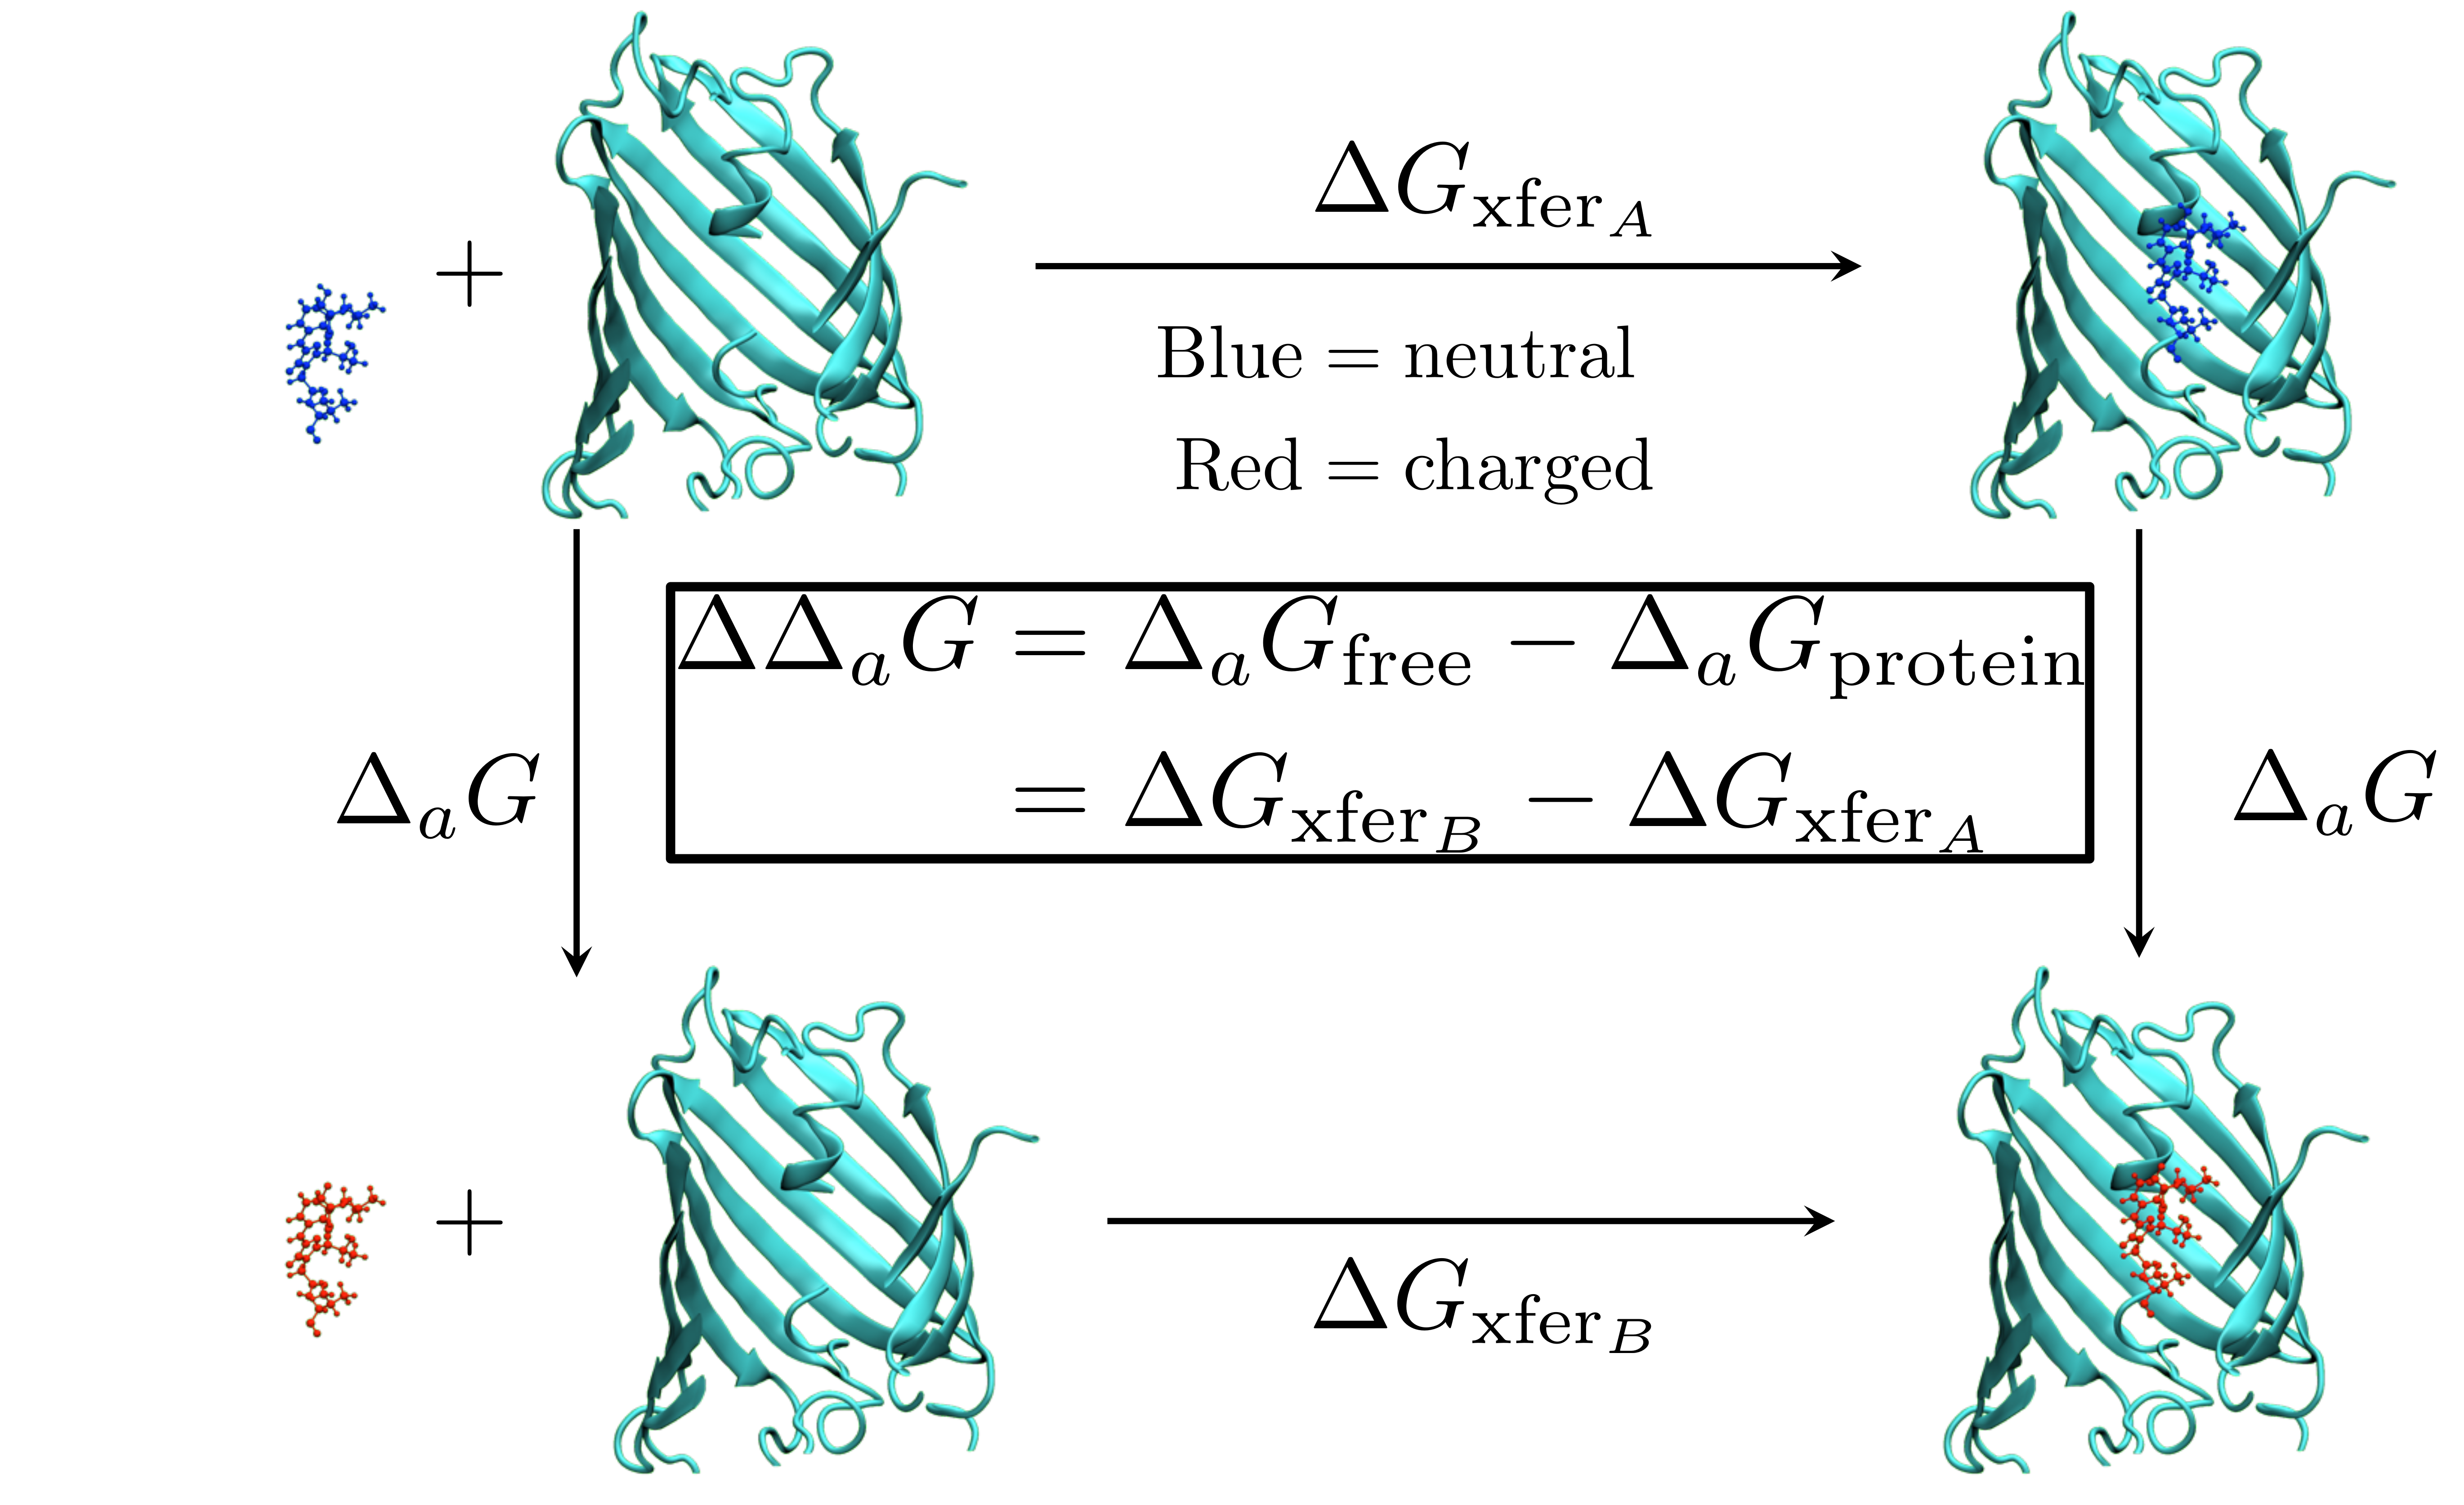
\includegraphics[width=3.25in]{figures-gfp-pKa/thermocycle.png}
    \label{fig:thermocycle}
    \caption{Cartoon representation of the thermodynamic cycle used for \pKa{} calculations. The A and B states of the fluorophore are shown in blue and red, respectively. The GFP structure is shown as a cyan cartoon.}
\end{figure}

Specifically, we wanted to evaluate the performance of APBS to reproduce the fluorophore \pKa{} values using minimal optimization to the commercially-available software package. 
We first performed the free energy calculations on the static starting structures that were modelled by homology from crystal structure 2b3p. 
The solvent was treated implicitly with a dielectric constant of 78.54 and the crystallized atoms were treated with a dielectric constant of 20, which is thought to be an effective protein dielectric in static structure calculations.24
While removing all explicit water molecules and replacing them with a continuum dielectric has been shown to be an accurate approximation in the continuum treatment of compact globular proteins,73,74 it may not necessarily hold for the $\beta$-barrel of GFP, which contains many confined water molecules that form intricate hydrogen bonded networks with other waters and protein residue side chains. These confined waters near the fluorophore likely play a large role in determining the \pKa{} through both structural and electrostatic effects.
Therefore, any crystallized waters within a 5 \si{\angstrom} sphere around the fluorophore phenol (or phenolate) oxygen were treated explicitly.
The results from these calculations are shown in Figure \ref{fig:calc_pKas}A, where we observed a poor correlation between the calculated and experimental \pKa{} values (r = 0.27).
We hypothesized that this was due to insufficient protein relaxation around the residue of mutation.
For example, inserting a nitrile probe at either position 145 or 165 often caused steric clash with nearby residues.
Molecular dynamics would add the protein relaxation into the model and eliminate this concern.
Additionally, we wanted to model protein fluctuations because PB-based calculations are extremely sensitive to protein configuration.

\begin{figure}
    \center
    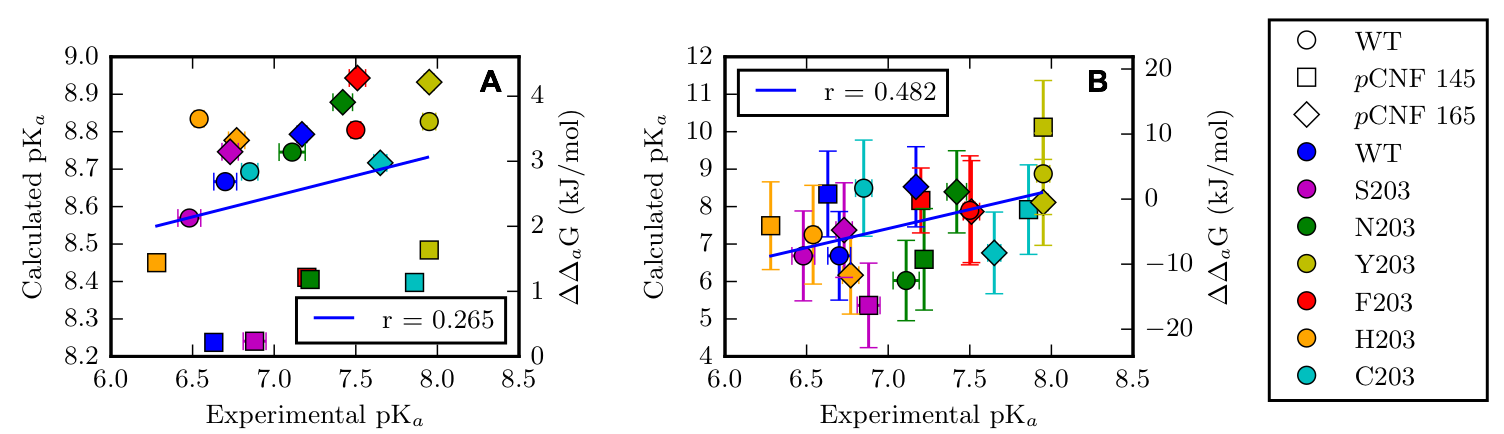
\includegraphics[width=6.0in]{figures-gfp-pKa/calc_pKas.png}
    \label{fig:calc_pKas}
    \caption{Correlations between experimentally measured \pKa{} values and those calculated in APBS. In both cases, the calculated \pKa{} is shown on the y-axis and the experimental \pKa{} is on the x-axis. Data points shown as circles represent the mutant constructs with no nitrile probe, squares are the mutants with \pCNF{} at position 145, and diamonds are the mutants with \pCNF{} at position 165. Error bars on the x-axis are small relative to the size of the data points. (A) Correlation between experimental and calculated \pKa{} for APBS calculations performed on the modeled starting structures with the inclusion of explicit water molecules within a 5 \si{\angstrom} radius of the phenolic oxygen of the fluorophore as described in the main text. (B) Correlation between experimental and calculated \pKa{} for APBS calculations performed on snapshots of 50 ns of MD simulation with the inclusion of explicit water molecules within a 5 \si{\angstrom} radius of the phenolic oxygen of the fluorophore.}
\end{figure}

To account for the sensitivity of the calculation to the protein configuration, we performed molecular dynamics (MD) simulations on the protein structures (including explicit solvation with TIP3P water) to generate an ensemble of reasonable structures that might exist during the course of a room temperature steady-state experiment.
We first wanted to validate our parameters for the GFP fluorophore and the surrounding titratable residues (namely E222 and H148) to ensure that the MD simulations gave a reasonable ensemble of protein configurations.
Specifically, for GFP mutants containing the TYG fluorophore (used in the present study), there is detailed crystallographic evidence of the complex hydrogen bonding network around the fluorophore, which we used as a basis for comparison for our ensemble of protein configurations.54 
Table SXX in the Supplementary Information lists 17 different hydrogen bonding interactions that were observed in the crystal structure of an analogous GFP mutant near the embedded fluorophore, as well as the corresponding interactions from our 50 \si{\ns} of MD simulation of wild type superfolder GFP.
We observed all 17 hydrogen bonding interactions in our simulations.
While most interactions were captured by the simulations to within < 1 \si{\angstrom} of the distances measured from the crystal structure, there were a few notable differences.
In our simulations, Q69 and Q94 were both further away from the fluorophore, which gave rise to interaction distances to the atoms in those residues that were greater than the distances predicted by the crystal structure.
This is likely due to the difference in amino acid sequence between the present study and the crystal structure that was used for comparison, or the fact that the crystal structure only represents a single, low energy conformation of the protein.
Interestingly, simulations with negatively charged E222 and H148 protonated at the N$_{\varepsilon}$ were not able to accurately reproduce these 17 hydrogen bonding interactions (data not shown).
Overall, the fact that our MD simulations were able to accurately capture most of the experimentally observed hydrogen bonding interactions around the fluorophore suggests that we used reasonable parameters for the GFP fluorophore and supports our decision to protonate E222 and the N$_\delta$ of H148.
However, there is no structural data available for any of the position 203 mutants or the mutants with \pCNF{} 145 or 165.

To further validate our model parameters for the fluorophore and positions 145, 165, and 203, we followed the RMS deviations of each mutant protein relative to its minimized starting structure over the course of a 50 \si{\ns} trajectory of MD simulation.
These results are shown in Figure SXX in the Supporting Information, where we observed that the backbone RMS deviations remained low (< 2.7 \si{\angstrom}) throughout the protein trajectory for all 42 simulations.
This suggests that single point mutations to position 203 and/or insertion of \pCNF{} at either position 145 or 165 did not cause major structural rearrangements to GFP.
Indeed, our RMS deviations are of the same order of magnitude observed elsewhere for simulations of GFP.55,75
We interpret this observation to conclude that the simulations accurately represent a stable state of the protein (compared to the stable state represented by the crystal structure), and that the amount of motion modeled in the protein over the course of the MD trajectory was consistent with previous simulations.
Although none of this implies these simulations have given a ``correct" ensemble of structures, they do give confidence that our mutations at positions 203, 145, and 165 do not cause long time-scale rearrangements of the protein backbone, and that our simulations are adequately modeling the fluorophore environment. 

Using these trajectories, we performed \pKa{} calculations on an ensemble of structures extracted at regular intervals from the MD simulations.
The first 10 \si{\ns} of each simulation were discarded as equilibration time, and an ensemble of 80 structures, each 500 ps apart, were used to calculate an ensemble average of fluorophore \pKa{} values.
For all MD simulations and \pKa{} calculations, we observed convergence of the ΔG values (and thus the predicted \pKa{}) over the course of 50 \si{\ns} (Figure S5).
We therefore determined that additional simulation time would not result in changes in the calculated \pKa{} values. 

We performed our \pKa{} calculations on each extracted frame and where we explicitly included any water molecules within a 5 \si{\angstrom} sphere of the phenolic oxygen of the fluorophore.
The explicit atoms (protein and water) were treated with a dielectric of 6, and any waters outside of this sphere were removed and replaced with a continuum dielectric of 78.54.
Thus, our calculations were insensitive to the location of origin of any particular water molecules, because they were allowed to move into and out of the 5 \si{\angstrom} sphere throughout the MD simulation.
The reduction of the dielectric constant to 6 for the explicit atom region (as opposed to 20 in the static structure calculation) accounts for the inclusion of protein dynamics in the model.
The results of these calculations are shown in Figure \ref{fig:calc_pKas}B, where we still observed a poor correlation to the experimental values (r = 0.48).
We explored the effect of different dielectric constants (between 2-8) for the explicit atom region, and observed that the value of the protein dielectric constant did not substantially affect the correlation to experiment (data not shown).
We decided 6 was the most appropriate dielectric constant for these calculations, as it best recreated a one-to-one correlation to the experimental \pKa{} values, and could account for the polarizability and other electronic properties of the protein.
Thus, those calculations, with protein dielectric of 6, are reported here.

The results of these calculations are shown in Figure \ref{fig:calc_pKas}B, where we observed still a poor correlation to the experimental values (r = 0.48).
Overall, our results suggest that simple continuum models, such as the one used here, are inadequate to describe the electrostatic heterogeneity of the interior of GFP.
Additionally, even when combined with expensive all-atom simulations with explicit water, the correlation to experiment does not significantly improve.
One potential shortcoming of this calculation method is that we have ignored any coupling between the titration states of the fluorophore and the surrounding titratable residues (most notably E222 and H148).
While there is indirect crystal structure evidence54 that E222 remains protonated in both the A and B states of the fluorophore, this may not necessarily hold true for all the mutant we investigated.
Further studies are underway to explore the effects of different spheres of inclusion of explicit waters,  and using different dielectric constants of protein, and titration state coupling between the fluorophore, E222, and H148.

Despite the inability of APBS to accurately reproduce these experimentally measured \pKa{} values, our data set is unique and offers benefits over current protein electrostatics benchmarks.
Here, we have made systematic mutations at a single site (position 203) near the same titration event (GFP fluorophore) that result in \pKa{} changes of nearly 2 pH units.
This is in contrast to traditional data sets of \pKa{} values measured at various sites throughout the entirety of globular proteins like Staphylococcal nuclease or lysozyme.27,76,77
While these traditional data sets allow for rigorous tests of \pKa{} prediction models, they are comprised of titratable residues that exist in environments that are drastically different in both solvent and protein environment, making it difficult to identify the causes of success and failure in \pKa{} predictions.
The systematic nature of these \pKa{} shifts in the unique, water-filled $\beta$-barrel of GFP could offer a convenient alternative benchmark. 

\subsection{Calculating Nitrile Electric Fields}

For 14 of these protein systems, a \pCNF{} residue at either position 145 or 165 was used as VSE reporter of electric field change based on Equation \ref{eq:stark}.
Because site-specific electric fields, specifically those projected along the nitrile bond axis of \pCNF{} 145 and 165, are easily accessible from our MD simulations, we wanted to test whether the absolute values of the measured nitrile frequencies were correlated to these calculated fields.
We chose to calculate the fields using the Reaction Field method, which has been described in detail elsewhere and is known to minimize the error implicit in integrating the PB equation.78
We performed the APBS electric field calculations on 80 frames collected every 500 ps from our all-atom, explicitly-solvated protein trajectories.
In accordance with the RF method, the protein was treated with a dielectric constant of 2 and all waters (except those within a 5 \si{\angstrom} sphere of the \pCNF{} probe) were replaced with a dielectric constant of 78.54.
Additionally, because we simulated the A and B states separately for each mutant, and the experimental frequencies were measured for proteins that exist in an equilibrium of A and B states, it was necessary to weight the trajectories in order to calculate fields which were consistent with our VSE measurements.
For all of the simulations, the average field converged to a single value during the course of the simulation (Figure S6).
Here, we report a weighted average of the A and B state fields at the midpoint of the nitrile bond, where the weights were assigned based on the experimental \pKa{} values and the Henderson-Hasselbach equation.
The individual fields for the A and B state of each mutant are shown in Figure S7, where we generally observed small differences in fields between the A and B state simulations compared to the size of electric field fluctuations.
The results of these field calculations are plotted against the experimental vibrational frequencies (determined from Figure \ref{fig:abs_spectra}D) in Figures \ref{fig:calc_forces}A and \ref{fig:calc_forces}B.
In both the case of the \pCNF{} 145 and 165 probes, the continuum based model again failed to describe the complex interior of GFP, with correlations to experiment of -0.05 and 0.41, respectively.
To test the sensitivity of these calculations to the salt concentration within the simulation box, we performed calculations with 12 and 24 additional sodium and chloride ions.
However, even at high salt concentrations, the calculated fields at the nitrile bond did not significantly change (data not shown).
We believe that a model that can accurately describe the polarity and polarizability of, as well as the specific hydrogen bonding interactions inside GFP will be necessary to accurately reproduce these experimentally measured nitrile frequencies.79
We are currently expanding our studies of these nitrile probes to locations other than 145 and 165 to test the general applicability of these continuum-based models to reproduce the measured nitrile frequencies.

\begin{figure}
    \center
    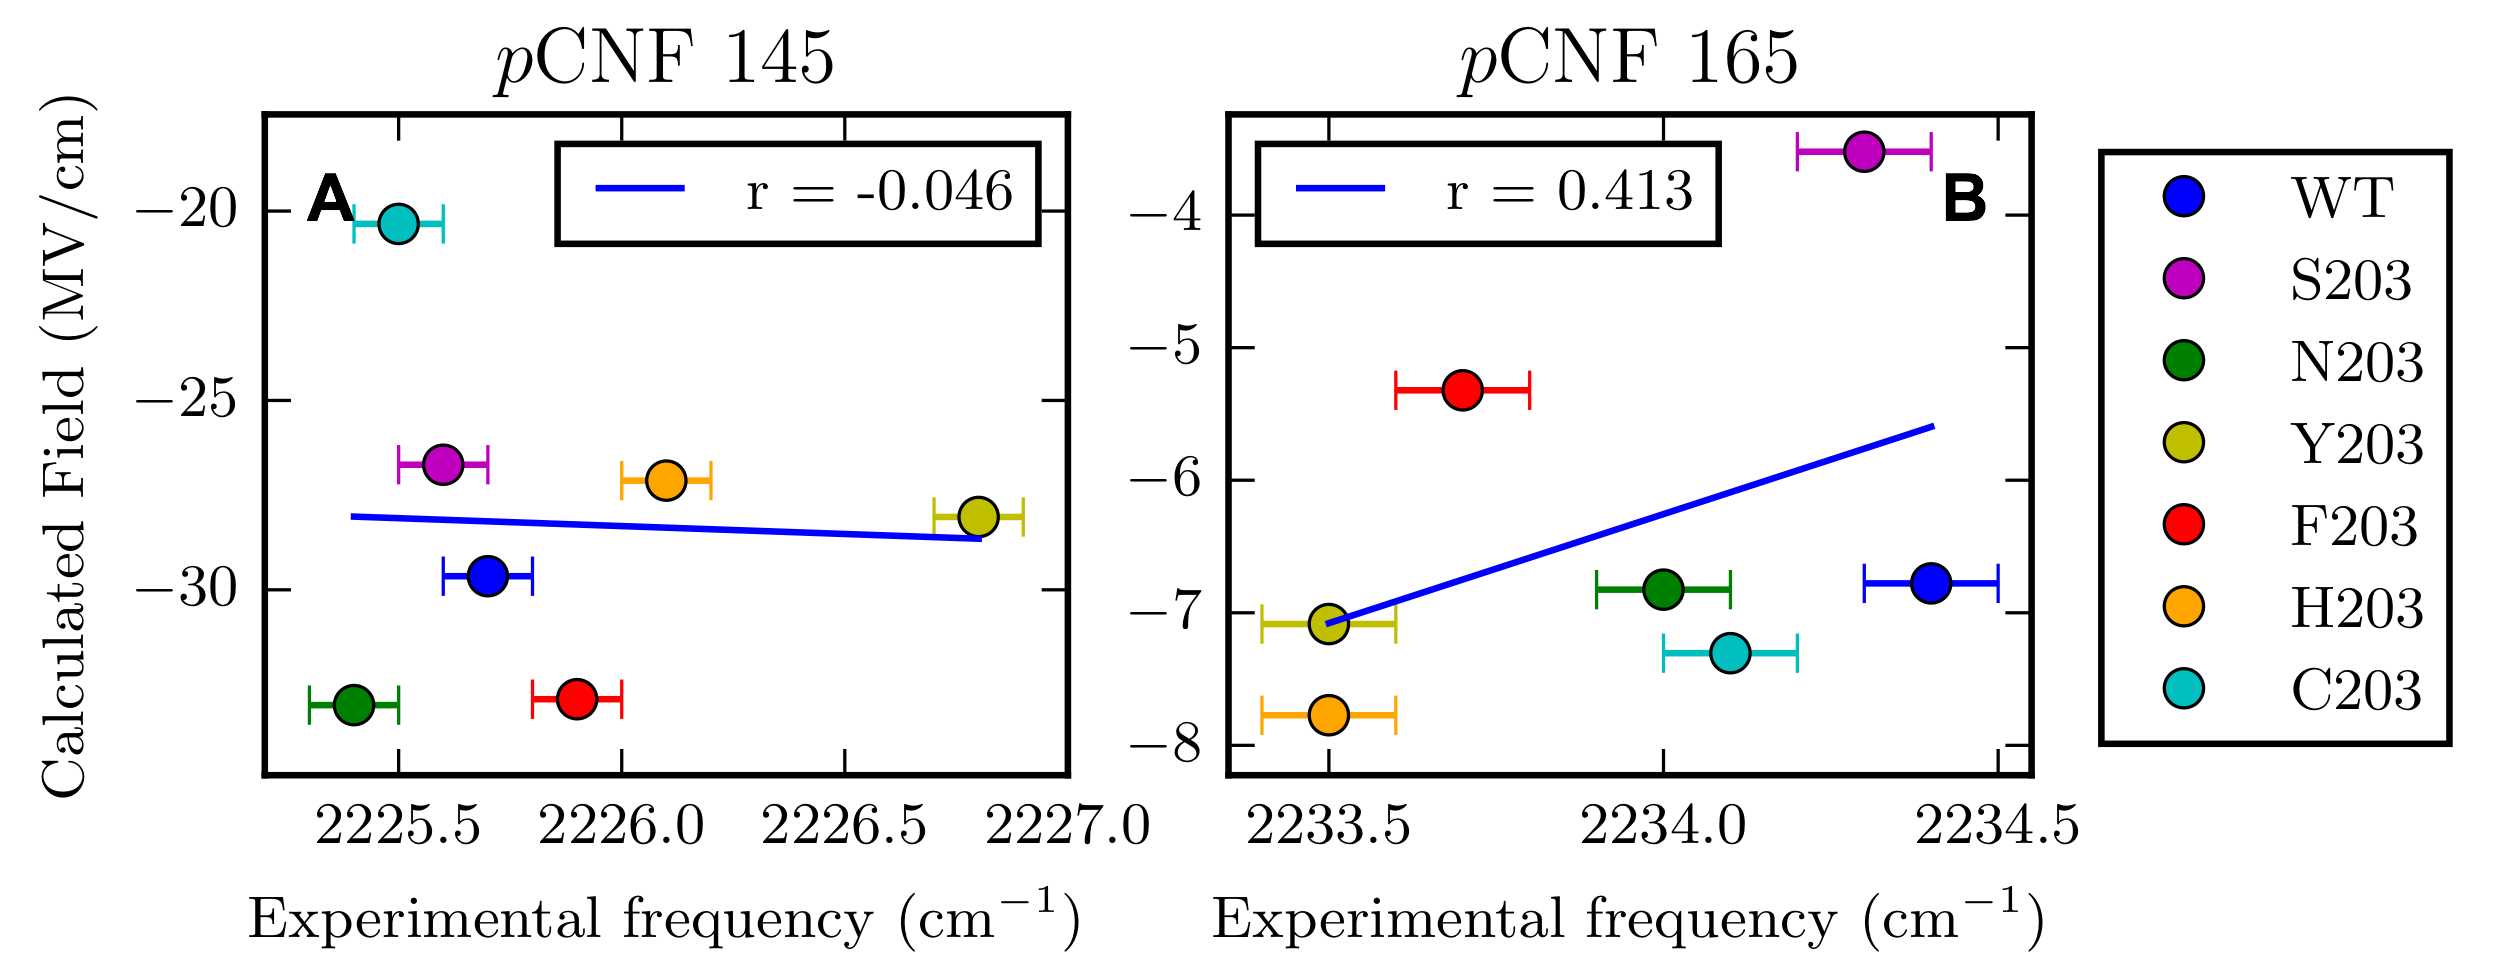
\includegraphics[width=6.0in]{figures-gfp-pKa/calc_forces.png}
    \label{fig:calc_forces}
    \caption{Comparison of the experimentally measured nitrile frequencies to calculated electric fields along the nitrile bond of \pCNF{} 145 and 165. Error bars on the y-axis have been omitted for clarity; in general, the distributions of fields calculated for each data point from the ensemble of MD structures are large relative to the shifts in average field ($\pm100\%$). (A) Calculated field using the APBS-based RF method along the bond vector of \pCNF{} 145 compared to the experimentally measured vibrational frequency. (B) Calculated field using the APBS-based RF method along the bond vector of \pCNF{} 165 compared to the experimentally measured vibrational frequency.}
\end{figure}

%%%%%%%%%%%%%%%%%%%%%%%%%%%%%%%%%%%%%%%%%%%%%%%%%%%%%%%%%%%%%%%%
%%%%%%%%%%%%%%%%%%%%%%%%%%%%%%%%%%%%%%%%%%%%%%%%%%%%%%%%%%%%%%%%
\section{Conclusions}\label{conclusion}
%%%%%%%%%%%%%%%%%%%%%%%%%%%%%%%%%%%%%%%%%%%%%%%%%%%%%%%%%%%%%%%%
%%%%%%%%%%%%%%%%%%%%%%%%%%%%%%%%%%%%%%%%%%%%%%%%%%%%%%%%%%%%%%%%


Here, we have shown that shifts in GFP fluorophore \pKa{} caused by nearby amino acid mutations are generally in good agreement with the corresponding Stark effect shifts of both the fluorophore and \pCNF{} probes inserted near the fluorophore.
This observed agreement between the vibrational and electronic Stark effect probes and \pKa{} shifts not only provides confidence in each of these measurements as probes of non-covalent environment, but also offers an unprecedented level of information about the electrostatic environment around the GFP fluorophore.
Because of this, we think the GFP fluorophore offers a unique benchmark for electrostatics models.
Contrary to datasets of \pKa{} values measured from titratable residues at various sites in the interior of a protein, we have measured \pKa{} shifts of a single interior site as a function of changes in local environment, caused by the position 203 mutations.
In addition to providing a range of \pKa{} values of the same residue as a function of nearby mutations, this dataset also offers the ability to benchmark electrostatics models against site-specific measurements of electric field changes that arise from the same mutations.
To test these possibilities, we used the popular APBS software package, coupled with MD simulations, to calculate the fluorophore \pKa{} values and the site-specific electric fields experienced by the nitrile probes.
We found that the continuum treatment of the GFP interior is insufficient to accurately reproduce the experimentally measured \pKa{} values and electric fields shifts.
In summary, we have reported that electrostatic perturbations, induced by mutations at position 203, cause similar changes in (1) the VSE shifts of inserted nitrile probes; (2) the electronic Stark effect shifts of the GFP fluorophore; and (3) the fluorophore \pKa{} values.
We suggest that the data presented here will be useful to other researchers, not only to validate protein electrostatic models, but also to elucidate the underlying physical determinant of fluorophore equilibrium in fluorescent proteins. 
